\documentclass[a4paper,11pt,french]{article}

\widowpenalty=9999
\clubpenalty=9999

\def\android{Android\texttrademark{}}

\usepackage[frenchb,english]{babel}
\usepackage[T1]{fontenc}
\usepackage[utf8]{inputenc}
\usepackage{um2/um2}
\usepackage{verbatim}
\usepackage{graphicx}
\usepackage{alltt}
\usepackage{enumitem}
\usepackage{tikz}
\usetikzlibrary{shapes,positioning,snakes,calc}

\usepackage{tikz}
\usetikzlibrary{shapes,positioning,snakes,calc}

\setlength{\parindent}{0pt}
\setlength{\parskip}{2ex}


\title{Rapport de TER
\\Master 1 Informatique
\\---\\
Reconception du jeu Pticlic sous \android{}}
\author{Yoann \textsc{Bonavero} \and Bertrand \textsc{Brun} \and John \textsc{Charron} \and Georges \textsc{Dupéron}}

\begin{document}

\maketitle

\pagenumbering{roman}
\pagestyle{empty}
\thispagestyle{empty}

\tableofcontents


\pagestyle{empty}
\thispagestyle{empty}
\newpage
\pagenumbering{arabic}
\setcounter{page}{1}
\pagestyle{plain}

\selectlanguage{frenchb}
\begin{abstract}
  PtiClic est un jeu de mots où des utilisateurs jouent et des données lexicales et sémantiques sont récoltées automatiquement ou
  semi-automatiquement. De telles approches pour peupler une base de données sont rapides, efficaces, peu coûteuses et présentent bien
  d'autres avantages. Dans PtiClic, les joueurs associent des idées à des mots et marquent des points si leurs réponses correspondent aux
  réponses d'autres utilisateurs. PtiClic est une application Web qui a été créée par Mathieu Lafourcade et Virginie Zampa.

  L'objectif du présent projet est de créer un prototype pour téléphones sous Android. Cette nouvelle version permettrait à des utilisateurs
  de jouer n'importe quand et n'importe où. Le sujet du projet a été élargi pour inclure une application qui pourrait fonctionner sur un
  grand nombre de téléphones mobiles et non pas seulement ceux sous Android. Les avantages, les inconvénients, les problèmes et les
  solutions associés à l'adaptation de ce jeu pour smartphone sont présentés dans ce document.
\end{abstract}

\selectlanguage{english}
\begin{abstract}
  PtiClic is a fun game word game in which users play and lexical and semantic data is collected automatically or semi-automatically. Such
  methods of populating a database are fast and inexpensive and have many other advantages. In PtiClic, players associate ideas with words
  and score points if their answers correspond to that of other users. PtiClic is a Web-based game which was created by Mathieu Lafourcade
  and Viginie Zampa.

  The purpose of this project is to create a prototype for telephones using the Android operating system. The application would permit users
  to play anywhere, anytime. The topic of the project was widened to include an application that can run on many different types of
  smartphones, not only those using the Android operating system. The advantages, drawbacks, problems and solutions associated with adapting
  the application for mobile phones are discussed throughout the document.
\end{abstract}
\selectlanguage{frenchb}
\pagebreak

\section{Introduction}

PtiClic\footnote{http://pticlic.org} est un jeu qui a été conçu et développé par Matthieu Lafourcade et Virginie Zampa. Le jeu a été créé afin de faire des études sur le vocabulaire et la sémantique sur des sujets de divers horizons dans un contexte ludique et motivant. Un mot central apparait, un nuage de mots entoure le mot central et le joueur clique et dépose des mots du nuage dans des catégories proposé sous forme d'énoncés. 

Par exemple, pour le mot central «bicyclette», les mots «pédale», «piéton», «pied», «automobile», «Sébastien Chabal», «Lance Armstrong», «pédalier», «voiture», «yeux», «rapide», «routier», «maillot», «pédaler», «dopage», «véhicule», «musclé», «nez», etc. sont proposés. Le joueur dépose ces mots dans les catégories «\dots{} est une partie de 'cycliste'», «Un contraire de 'cycliste' est \dots{}», «'cycliste' a un rapport avec \dots{}»,  «Une caractéristique de 'cycliste' est \dots{}» ou aucune de ces catégorie. Un score est obtenu en soustrayant les mots manquants et les mots incorrects aux mots corrects. 

Des linguistes et des informaticiens récupèrent les données liées aux parties jouées, ce qui leur permet de faire de la recherche dans leurs domaines respectifs.

Notre travail consiste à créer une version du PtiClic sous \android{}, une version modifiée du jeu adaptée pour téléphone mobile. Le sujet du TER définit clairement l'objectif de ce projet~:

\begin{quotation}
\noindent  L'étude et le prototypage d'une version fonctionnant sur \android{} semble intéressante. En particulier on s'intéressera à deux aspects :
  \begin{itemize}
  \item les contraintes imposées par l'environnement smartphone
  \item le biais qu'imposent ces contraintes sur le jeu et les données récoltées.
  \end{itemize}
  
\noindent  Il s'agira donc de modéliser une version adaptée aux smartphones et d'en implémenter un prototype fonctionnel.
\end{quotation}

Dans un premier temps, une version de base a été conçue et réalisée. Ensuite, il a été prévu d'ajouter des fonctionnalités supplémentaires. La démarche adoptée par notre groupe a été une approche itérative. Initialement, quatre itérations et quatre livraisons devaient donner comme résultat une version de base et des versions plus élaborées~: un joueur pourrait, entre autres, modifier ses préférences ou choisir son niveau. L'idée était aussi de rendre le jeu plus attirant afin d'accroître le nombre de sujets participant aux études liées au résultat des données extraits des parties jouées.

Nos objectifs initiaux ont été modifié, nous avons créé deux prototypes, l'une sous Android en Java, l'autre en HTML5 élargissant notre public leur donnant la possibilité de jouer au jeu sur divers types de smartphones.  


\pagebreak

 
\section{Analyse de l'existant}

L'application du jeu du PtiClic d'origine est une application disponible en ligne sur \url{http://www.lirmm.fr/pticlic/pticlic.php}. Lors de
la réalisation de ce projet, nous n'avions pas accès au code source de l'application ni à des diagrammes UML. La seule partie de cette
application qui nous a été fournie est une archive de la base de données dans un format textuel.

L'analyse de l'existant consistait donc d'une analyse du format et du contenu de cette archive ainsi que l'application sur Internet que nous avons testé et analysé. Il était également possible d'avoir d'autres informations concernant l'application Web PtiClic à travers de nombreux articles écrits sur ce sujet et en communiquant avec les créateurs du jeu.

\subsection{Le déroulement du jeu}

L'utilisateur clique sur le bouton «Je joue !». Un mot\footnote{Pour simplifier l'écriture, nous parlons de 'mots', mais un mot peu aussi être un mot composé, un syntagme ou une phrase, y compris des noms propres.} se dirige vers le centre de la page, c'est le «mot central». D'autres mots viennent entourer le mot central, ce sont les «mots nuage». La police du mot central est plus grande que celle des mots nuages. Le mot central et les mots du nuage sont de couleurs contrastées.

\subsubsection{L'écran du jeu}
\begin{center}
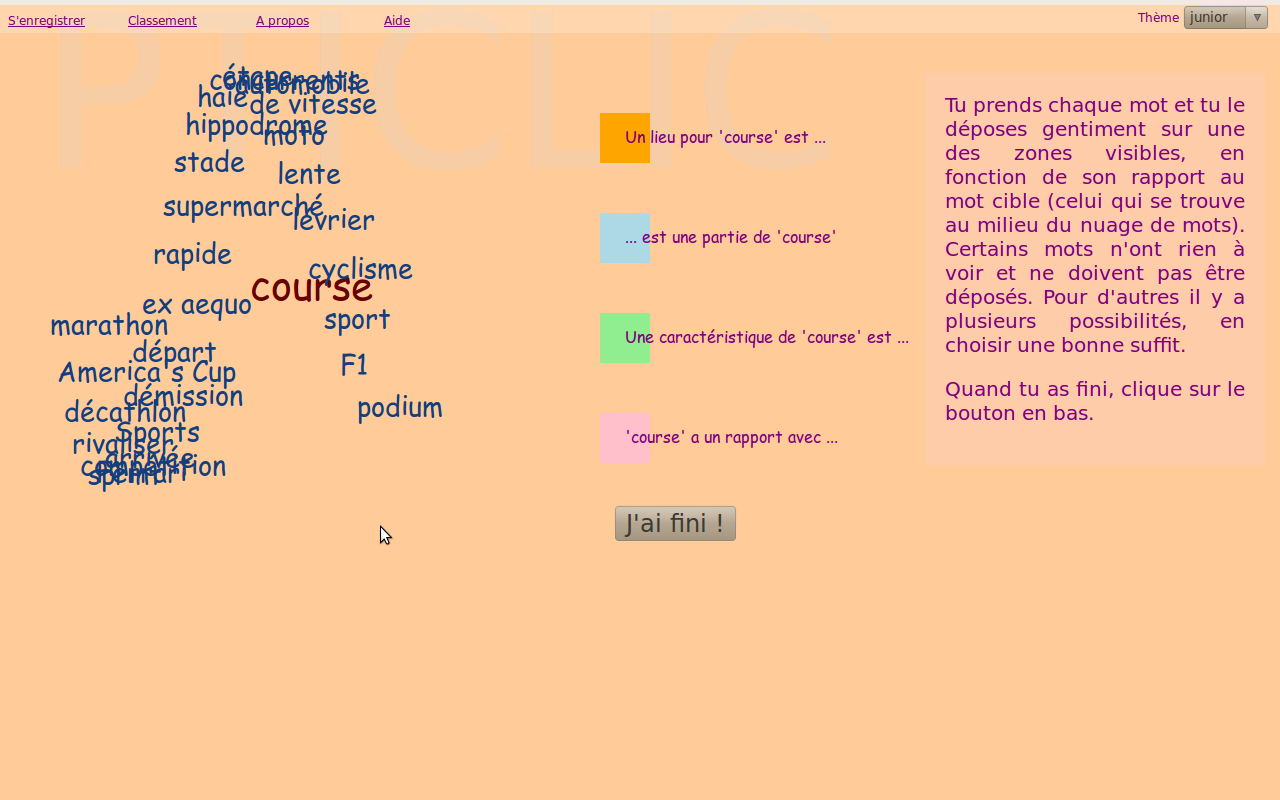
\includegraphics[width=14cm]{img/PtiClicJeu.png}
\end{center}

Les relations apparaissent à droite des mots. Une partie peut comporter d'une à quatre relations. Un carré apparaît à droite de la relation suivi de la relation sous forme de syntagme tel que «\emph{(mot central)} est en rapport avec\dots{}», «Quoi/Qui pourrait \emph{(mot central)}~?». S'il y a plus d'une relation, les relations apparaissent les unes en dessous les autres, toujours à droite des mots.

Encore plus à droite, un bref explicatif du principe du jeu, et tout en bas, le bouton «J'ai fini~!», 

Le principe du jeu est simple. Lorsque l'utilisateur estime qu'un mot nuage est lié au mot central par une des relations, il glisse et dépose le mot nuage sur le carré de la relation. Si l'utilisateur pense qu'aucune des relations ne convient, il laisse le mot dans le nuage tout simplement. 

\subsubsection{Déroulement de la partie}
\begin{center}
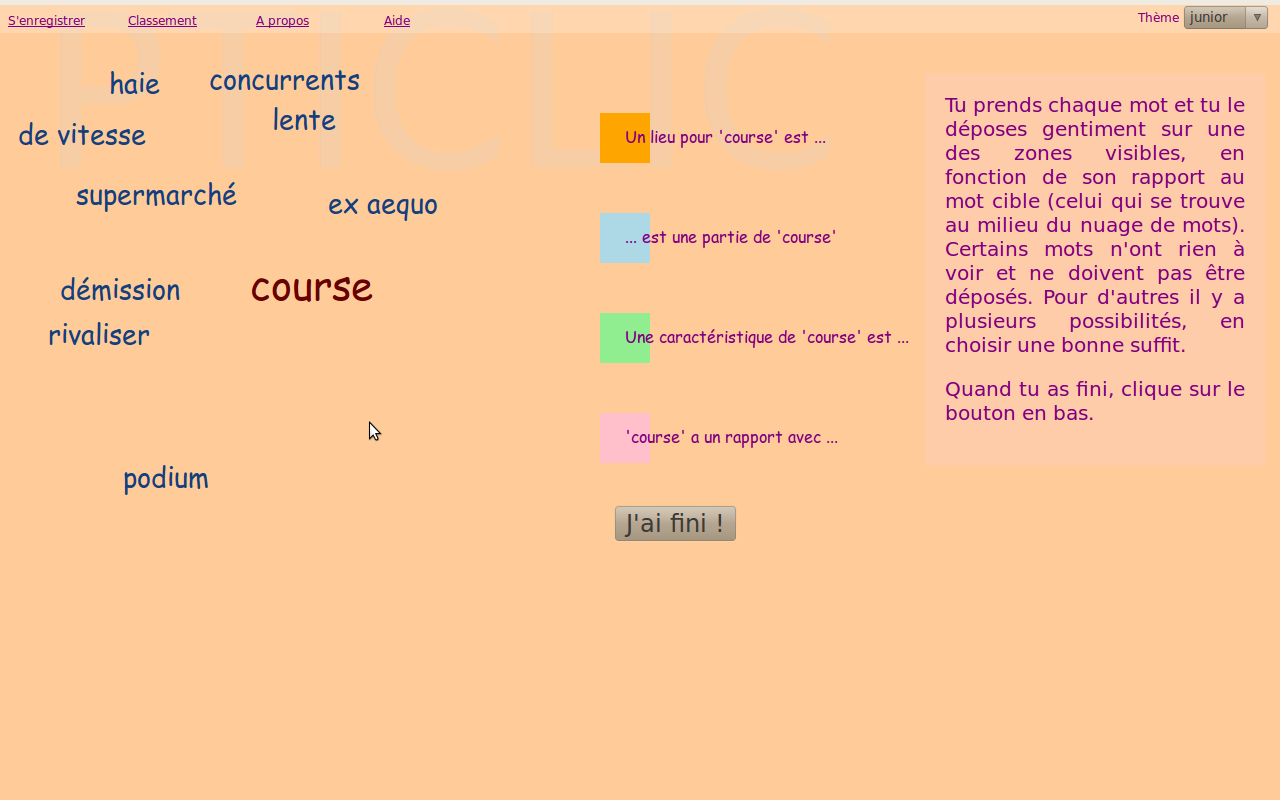
\includegraphics[width=14cm]{img/PtiClicJeu2.png}
\end{center}

Si le joueur se trompe, il peut double-cliquer sur le carré pour extraire le dernier mot déposé. En fait, le joueur peut double-cliquer
autant de fois qu'il le veut pour extraire tous les mots ayant été mis dans la relation un par un afin de modifier ses choix. Lorsque le
joueur a fait ses choix et souhaite terminer la partie, il clique sur «J'ai fini~!», ce qui le renvoie vers la page des résultats et du
score. Il n'y a aucune limite de temps pour terminer une partie.

\subsubsection{Score obtenu}
\begin{center}
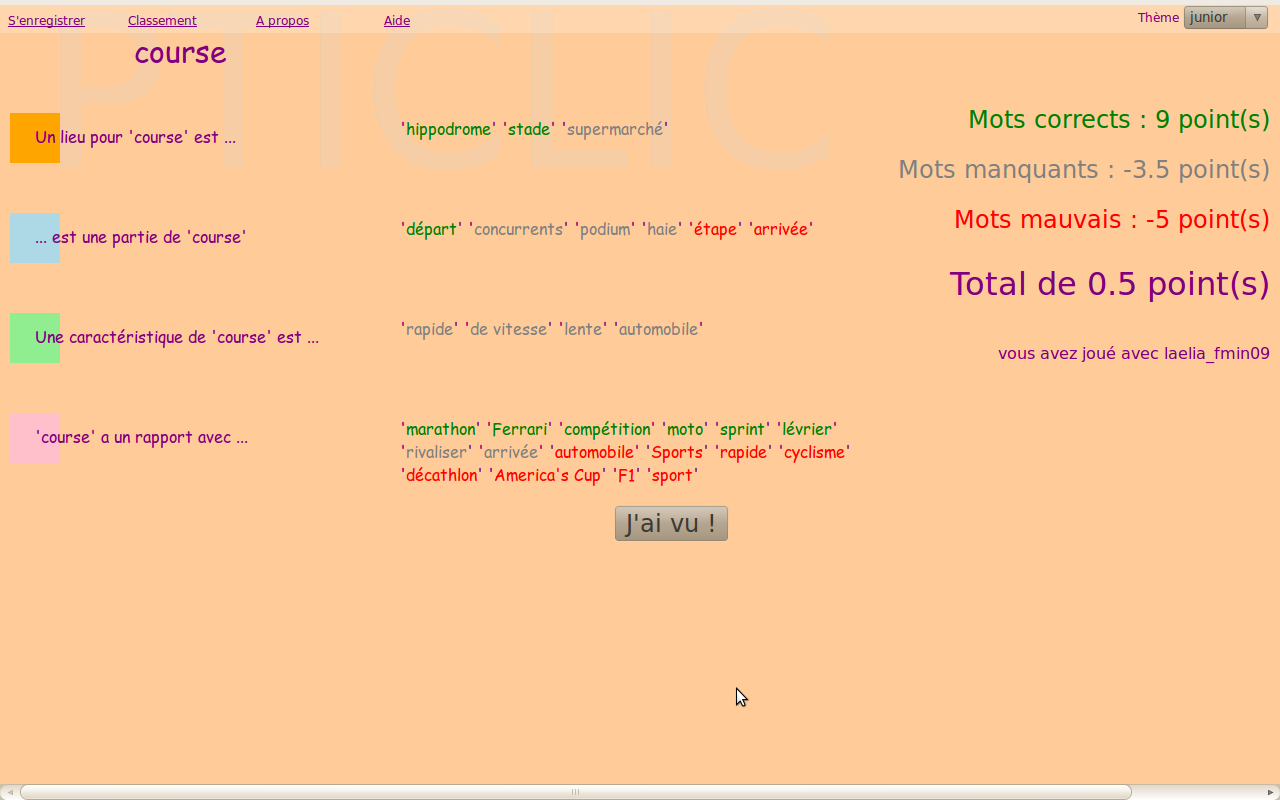
\includegraphics[width=14cm]{img/PtiClicResultats.png}
\end{center}

La page des scores contient aussi le corrigé de la partie\footnote{Un joueur joue contre un autre joueur. Le «corrigé» contient donc les réponses qui correspondent à celles du joueur contre qui il joue. En conséquence, une «bonne» réponse peut correspondre à deux mauvaises réponses, mais qui ont été choisit par les deux joueurs en question. Toutefois, le poids des relations augmentent seulement si plusieurs paires de joueurs donne les mêmes réponses.}. Les mots qui ont été mis dans la bonne categorie apparaissent en vert, les
mauvaises réponses en rouge et les omissions en gris. Un point est marqué par bonne réponse tandis qu'une mauvaise réponse ou une omission
fait perdre un demi-point. Lorsque deux réponses sont possibles, le point est marqué quelque soit la relation choisie. Le score final est
soit un entier, soit un entier plus un demi point~; il peut être négatif, nul ou positif.

Lorsque l'on clique sur le bouton «J'ai vu !», on retourne sur la page d'accueil.

\subsubsection{L'écran d'accueil du site}
\begin{center}
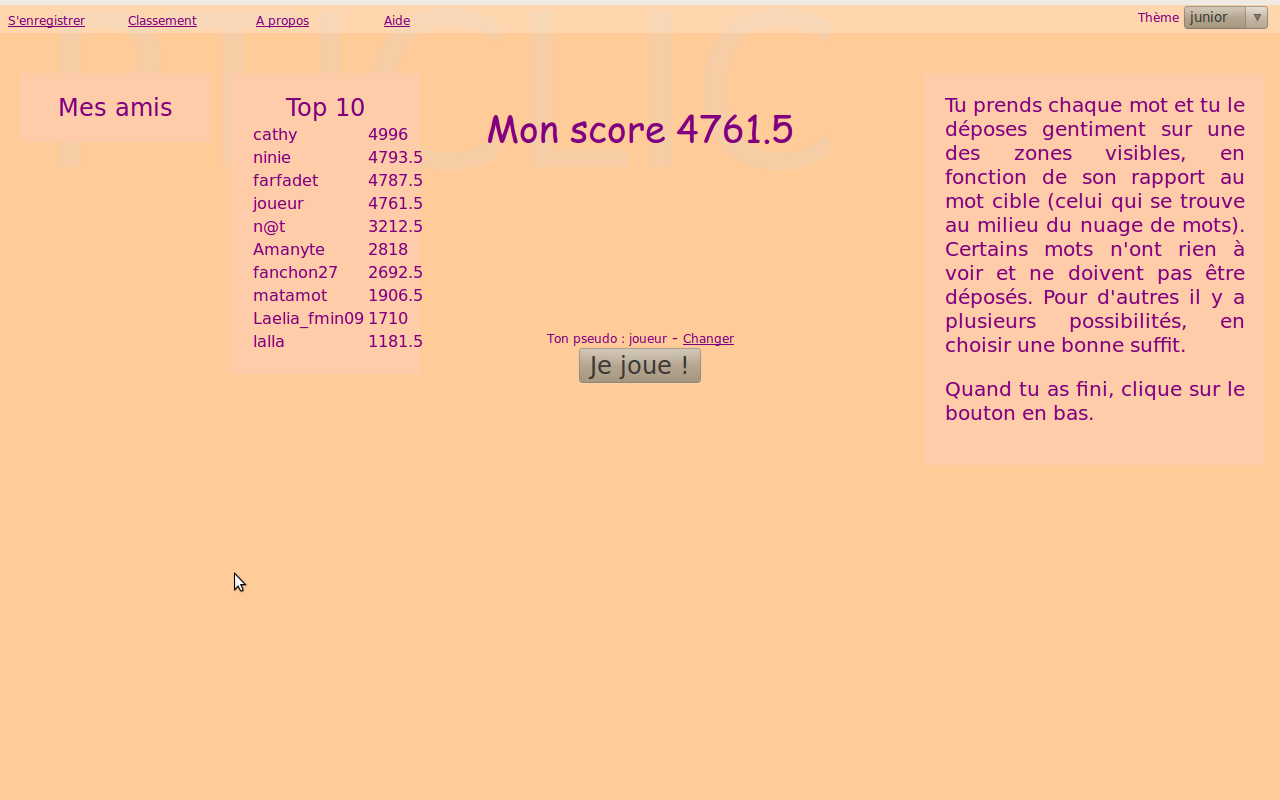
\includegraphics[width=14cm]{img/PtiClicAccueil.png}
\end{center}

Le joueur par défaut est l'utilisateur "joueur". Il est aussi possible de s'inscrire sur le site afin de créer son propre identifiant et mot
de passe afin de cumuler des points à chaque partie joué. Les dix joueurs qui ont cumulé le plus grand nombre de points sont inscrits sur la
liste des «Top 10». Les points cumulés par le joueur «joueur», qui est l'ensemble de parties jouées par des internautes non inscrits au
site, figure parmi les «Top 10». A droite de ceci, le score du joueur en question, c'est-à-dire, la somme totale des scores de toutes les
parties jouées par l'utilisateur. Si l'utilisateur veut jouer une partie de plus, il clique sur le bouton «Je joue~!» en bas de la page et
une nouvelle partie est entamée.

Huit styles de couleurs sont disponibles et modifiables dans le menu déroulant en haut à droite de la page d'accueil. D'autres modifications résultent lors d'un changement de style, par exemple, les phrases associées aux relations. Lorsque le joueur s'authentifie avec succès, son identifiant apparaît dans le fond de page en très grande taille.

Lorsqu'un utilisateur souhaite s'inscrire au site, il est invité à lire un document explicatif de l'objectif du jeu dans le cadre du projet
de recherche de ce dernier. Il est aussi averti du contenu potentiel du jeu : comme les mots centraux et du nuage sont fournis par d'autres
utilisateurs, le vocabulaire rencontré peut ne pas convenir aux moins de 16 ans.



\subsection{L'archive de la base de données}

L'archive de la base de données est un fichier plat d'environ 2 000 000 lignes. Ce fichier contient un grand nombre de caractères accentués et
la version à notre disposition lorsque nous avons commencé à l'analyser, en extraire des données puis à créer notre propre base de données
n'était pas encodée en UTF-8.

La base de données de laquelle est extraite ce dump provient d'un autre jeu de l'équipe TALN\footnote{Traitement Automatique du Langage Naturel, NLP en anglais, Natural Language Processing} du Lirmm, nommé JeuxDeMots. L'objectif principal de JeuxDeMots est d'ajouter des mots et des expressions au réseau lexical alors que l'objectif principal de PtiClic est d'accroître le nombre de relations sémantiques entre les mots du réseau.

L'archive contient en tout début des remerciements et quelques explications des acronymes et des abréviations utilisés, puis des statistiques, à savoir, le nombre d'occurrences de relations, la fréquence des noeuds, les 50 termes les plus fréquents. Plus un terme ou expression est fréquent, plus son poids est élevé. 

L'archive a proprement parler contient deux grandes parties~: une partie 'noeuds' (\verb!NODES!) et une partie 'relations' (\verb!RELATIONS!). La partie 'noeuds'  contient sont de divers types. Les noeuds de type 'terme' contiennent non seulement des adjectifs, des adverbes, des substantifs et des verbes, mais aussi des locutions et des syntagmes, des mots tels que les prépositions, les conjonctions, les pronoms, les articles et les déterminants. Les substantifs peuvent être des noms propres, y compris des noms de lieux, des noms de personnes. Il existe de noeuds qui donnent d'autres informations, et on verra plus tard que ceux qui nous intéressent le plus, outre les termes, sont ceux concernant la catégorie grammaticale des mots et d'autres informations métalinguistiques plus précises.

Dans la partie 'mots et expressions', chaque entrée -- chaque ligne -- contient un $eid$ (Entry IDentifier), un nom $n$ (name), un type $t$ et un poids $w$ (weight). En voici un exemple~:
\indent%
\begin{verbatim}
eid=231064:n="pour femme":t=1:w=50
\end{verbatim}

Pour la partie relation, l'identifiant est le $rid$ (Relation IDentifier), le noeud de début $n1$ (starting node), le noeud de fin $n2$ (ending node), le $type$ (relation type) et le poids $w$ (weight). En voici un exemple~:
\begin{verbatim}
rid=430049:n1=82029:n2=151553:t=12:w=18
\end{verbatim}

\subsection{Analyse plus approfondie du jeu}
Bien que l'archive de la base de données contienne 55 relations différentes, la version en ligne du jeu du PtiClic n'en utilise que treize (uniquement celles qui sont pertinentes pour le jeu)~:

\begin{itemize}
\item r\_associated|0|idée|Tout terme lié d'une façon ou d'une autre au mot cible\dots{} Ce mot vous fait penser à quoi~? 
\item r\_syn|5|synonyme|A partir d'un terme, il est demandé d'énumérer les synonymes ou quasi-synonymes de ce terme. \item r\_isa|6|générique|'animal' est un générique de «chat', «mammifère', «être vivant' etc. en sont d'autres\dots{}
\item r\_anto|7|contraire|'chaud' est le contraire de «froid', vous vous rappelez~? :)
\item r\_hypo|8|spécifique|'mouche', «abeille', «guêpe' sont des spécifiques de «insecte»\dots{}
\item r\_has\_part|9|partie|Il faut donner des parties/constituants/éléments du mot cible. Par exemple, «voiture» pourrait avoir comme parties : «porte», «roue», «moteur»\dots{}
\item r\_holo|10|tout|Le tout est ce qui contient l'objet en question. Pour «main', on aura «bras', «corps', «personne', etc. On peut aussi voir le tout comme l'ensemble auquel appartient un élément, comme «classe' pour «élève'.
\item r\_agent|13|action>agent|L'agent (qu'on appelle aussi le sujet) est l'entité qui effectue l'action. Par exemple dans - Le chat mange la souris -, l'agent est le chat. Des agents typiques de «courir» peuvent être «sportif», «enfant»\dots{} 
\item r\_lieu|15|chose>lieu|A partir d'un nom d'objet (ou autre), il est demandé d'énumérer les lieux typiques où peut se trouver l'objet en question.
\item r\_instr|16|action>instrument|L'instrument est l'objet avec lequel on fait l'action. Dans - Il mange sa salade avec une fourchette -, fourchette est l'instrument. Des instruments typiques de «tuer» peuvent être «arme», «pistolet», «poison»\dots{}
\item r\_carac|17|caractéristique|Pour une terme donné, en général un objet, il est demandé d'énumérer les caractéristiques possibles et/ou typiques de cet objet. Par exemple, pour «eau' on pourra avoir «liquide', «froide', «chaude', etc.
\item r\_lieu\_action|30|lieu>action|A partir d'un lieu, énumérer les action typiques possibles dans ce lieu.
\item r\_action\_lieu|31|action>lieu|A partir d'une action (un verbe), énumérer les lieux typiques possibles où peut être réalisée cette action.
\end{itemize}

Pour un mot central donné, seulement un nombre limité de relations sont possibles. Les adverbes et les locutions adverbiales sont relativement peu fréquents. La grande majorité des mots sont des substantifs, des verbes et des adjectifs ainsi que des locutions nominales, verbales et adjectivales. La relation "patient" est possible pour un mot central qui est un verbe, mais elle est plus complexe car elle ne fonctionnera que si le verbe en question est transitif. 

\pagebreak

\section{Analyse des besoins}

Comme tout outil, l'environnement smartphone présente à la fois des avantages et des inconvéniants. 

Les avantages sont nombreux~: un instrument portatif avec un bref temps de démarrage adapté à effectuer des tâches ponctuelles souvent de courte durée avec un écran tactile permettant d'agir directement sur des éléments affichés sur son écran. Le smartphone présente encore d'autres avantages, il est à la fois un lecteur mp3, un dictaphone, un appareil, un chronomètre et réveil, pour ne citer que quelques exemples.

Les inconvénients par rapport à un ordinateur classique sont aussi nombreux. L'écran est nettement plus petit limitant l'espace de travail
et obligeant davantage de navigation de page en page. L'entrée des données est plus difficile, il n'existe pas de clavier, ou bien seulement
un clavier virtuel ou un micro-clavier intégré. Malgré les avantages de l'écran tactile, son utilisation permet une précision bien moindre
que l'utilisation d'une souris à cause de la petite taille de l'écran et des doigts et mains qui bloquent la vue de l'écran lors du
glissement-et-déposé par exemple.

Le faible espace de stockage et les limites d'autonomie et d'énergie se traduisent par une nécessité d'économie de la part des concepteurs
d'applications par rapport aux ordinateurs classiques, de plus en plus performants actuellement. C'est pour cette raison que le smartphone
n'est pas le plus adapté pour effectuer des tâches de longue haleine telles que la rédaction des textes ou l'édition de vidéos. Notamment, dans notre cas,
l'utilisation du réseau est lente, potentiellement coûteuse pour l'utilisateur -- les forfaits facturant souvent à la quantité de données -- et
consommatrice d'énergie.

Les applications bien adaptées au smartphone sont des applications telles que les calculatrices, les logiciels de prise de notes, les jeux
simples (casual games) et le jeu du PtiClic n'est pas une exception à cette dernière catégorie. L'avantage de ces applications sur un smartphone est
qu'il est possible d'y jouer lorsque l'on est en file d'attente à la Poste ou à la Préfecture ou bien dans les transports en commun. En effet, lorsque l'on a un smartphone, on peut jouer n'importe quand et n'importe où. Un tel
prototypage du jeu demande toutefois une réflexion non seulement quant aux limites d'un smartphone mais aussi ses avantages.

Le jeu de base du PtiClic sous \android{} présente plus ou moins les mêmes cas d'utilisations que l'application d'origine. Toutefois, le 'comment' de ces cas d'utilisation sont loin d'être les mêmes, la plus grande différence étant la gestion des mots nuage. Une discussion de ce sujet fera l'objet des chapitres 'Conception' et 'Réalisation'.

\pagebreak

\section{PtiClic et le TALN}


Les projets JeuxDeMots et PtiClic s'inscrivent dans le domaine de la recherche en traitement automatique du langage naturel, et plus précisément dans celui du traitement de la sémantique du langage. Les données et les conclusions issues de ces projets pourraient contribuer directement ou indirectement à la recherche et à des applications en traduction automatique, l'indexation des textes, les correcteurs automatiques d'orthographe et de grammaire, la classification et la catégorisation des documents, des algorithmes de moteurs de recherche.


\subsection{Ferdinand de Saussure, la linguistique moderne, le TALN, JeuxDeMots et PtiClic}

Dans la partie qui suit, des notions de linguistique générale seront évoquées suivies d'une discussion d'applications dans le traitement automatique du langage naturel~: les dichotomies signifié-signifiant, langue et parole, synchronie et diachronie et l'arbitraire du signe. C'est Ferdinand de Saussure (1857-1913), fondateur de la linguistique moderne, qui a défini formellement pour la première fois ces concepts fondamentaux dans son Cours de linguistique général\footnote{Ferdinand de Saussure, Cours de linguistique générale, édition originale~: 1916, édition 1979~: Payot, Paris. Il s'agit d'une oeuvre posthume rédigée à partir de notes de cours par deux disciples de Saussure~: Charles Bally et Albert Sechehaye. La publication de cet ouvrage marque le début de la linguistique moderne.}.

\subsubsection{Le signe linguistique~: signifié, signifiant, référent}

Selon Saussure, le signe linguistique est une entité à deux faces~: le signifiant et le signifié. Ce principe semble assez simple. A un mot est associé un concept. Le mot 'cheval', c'est-à-dire son occurence orale ou écrite, le signifiant,\footnote{Pour Saussure, le signifiant est la version phonique d'un mot, ce qui est logique car la version graphique du mot n'est qu'une représentation écrite de la version phonique} nous évoque la représentation mentale que nous avons d'un cheval, le signifié. 


\begin{figure}[h!]
  \centering
      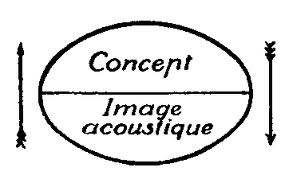
\includegraphics[width=0.5\textwidth]{img/signe-conceptimageacoustique.jpeg}
  \caption{Une représentation d'une idée, d'une chose, etc. est associée à la forme phonique d'un mot.}
\end{figure}

\begin{figure}[h!]
  \centering
      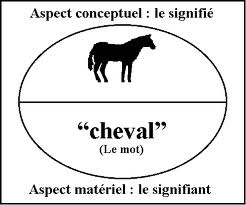
\includegraphics[width=0.5\textwidth]{img/signe-cheval.jpeg}
  \caption{A la représentation qu'on a d'un cheval est associé la forme phonique du mot cheval}
\end{figure}

Cette notion semble assez simple mais, au contraire, la relation signifié-signifiant est très complexe. Cette entité a un très grand nombre de caractéristiques et le signifiant comprend des dénotations ainsi que des connotations qui peuvent être liées à des contextes multidimensionnels, généraux et spécifiques. Puis, à la notion de concept s'ajoute l'objet lui-même... s'il s'agit d'un objet physique~! Et s'il s'agit d'une émotion~? D'une action~? D'un sentiment~? D'une idée abstraite~? 


On peut aussi parler de sens figuré et de sens propre des mots. Par exemple au mot «poésie» on pourrait associer les idées «littérature», «écrivain», «auteur», «strophes», etc. mais aussi «musique», «rêve», «amour». On parlera de ce deuxième sens lorsque l'on parle de la notion de «bruit» dans la relation entre mots ou expressions. Et si on prenait en compte la polysémie d'un signifiant~?


Un demi-siècle plus tard, Emile Benveniste ajouta une autre dimension à ce schéma intégrant un 'référent' qui remplace le 'signifié', le 'signifié' étant, pour Benveniste, la dénotation du mot, c'est-à-dire bien l'objet lui-même. 

\begin{figure}[h!]
  \centering
      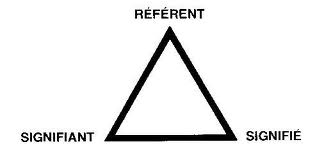
\includegraphics[width=0.5\textwidth]{img/trianglesemiotique.jpeg}
  \caption{Le signifiant de Saussure correspond au référent de Benveniste, le signifiant de Benveniste étant la dénotation du signifié alors que le référent est la représentation mentale ou 'concept' du signifié, qui englobe aussi des connotations qui peuvent être de nature très étendues telle que les contextes et les expériences personnelles que quelqu'un associe à un signifié.}
\end{figure}

Bien que ce modèle soit plus complet, cet ajout ne simplifie en rien notre travail. 

Un des obectifs des projets JeuxDeMots et PtiClic est d'établir des informations complexes concernant la représentation mentale d'un signifiant à travers ses liens avec d'autres signifiants. Bien que le langage soit limité, le langage demeure un des moyens de communication les plus efficaces de l'homme.\footnote{'Un' des moyens les plus efficace car les images, les vidéos, etc. sont aussi des moyens de communication qui peuvent être aussi efficace que le langage. Cependant, dans la majorité des cas, le langage reste un mode de communication qui permet de s'exprimer avec le plus de précision} 

Dans le réseau lexical JeuxDeMots, le signifiant est élargi pour comprendre non seulement des mots mais aussi des locutions, des expressions et des raffinements sémantiques. Lorsqu'un mot est polysémique, il peut avoir plusieurs entrées distinctes. Par exemple, pour le mot 'boîte', on trouve 'boîte (contenant)', 'boîte (entreprise)', 'boîte (de nuit)', 'boîte (conserve)', etc.

On verra que, dans le réseau lexical JeuxDeMots/PtiClic, il est possible de décrire à l'aide d'autres mots un grand nombre de traits sémantiques d'un signifiant au moyen d'un nombre assez important de relations que ce signifiant entretient avec d'autres signifiants (relations sortantes). Qui plus est, les traits sémantiques du signifiant en question sont encore élargis car il est aussi possible de lui associer des signifiants dont il fournit des traits sémantiques (relations entrantes). 

\subsubsection{L'arbitraire du signe}

A l'exception de quelques onomatopées, le lien entre un mot (sous forme orale ou écrite) et son concept est complètement arbitraire. Le mot pour 'arbre' en anglais est 'tree', 'Baum' en allemand. Il n'y a aucun rapport entre la représentation phonique ou graphique d'un mot et sa signification.

Le fait que le signe linguistique est arbitraire rend le travail des chercheurs et des informaticiens en TALN bien plus difficile. Aucun élément dans le mot écrit (qui représente sa forme orale), ou plutôt d'une famille de mots, nous donne des indices quant au sens d'un mot. Il est toutefois possible de déduire le sens d'un mot à partir d'autres mots apparentés ou en se servant des notions d'étymologie provenant d'autres languages (par exemple, le latin et le grec) ou issues de la même langue. Cependant, cela peut aussi donner lieu à des faux amis ou des faux apparentés. 

Ce fait peut sembler évident, mais il est bon d'en être conscient. En effet, si le signe linguistique n'était pas arbitraire, il serait théoriquement possible d'écrire un algorithme pour déduire le sens d'un mot à partir du signifiant, c'est-à-dire le signifié à partir du signifiant, ce qui n'est pas le cas, d'où la complexité du problème que pose la sémantique. 


\subsubsection{Synchronie et diachronie}

La notion de synchronie correspond à l'étude ou l'analyse d'une langue à un moment donné, figé dans le temps. La diachronie, elle, s'intéresse à l'évolution d'une langue.

Quoiqu'il soit intéressant d'étudier une langue à un moment donné dans le temps, cela ne correspond pas au monde réel. Une langue évolue quotidiennement grâce à ou à cause des nouveaux produits introduits sur le marché et les événements politiques du monde entre autre. Il est donc important de pouvoir tenir compte de ces changements. Ils sont pris en compte dans la base de données de JeuxDeMots grâce au fait que le réseau lexical évolue en temps réel ; le jeu qui alimente ce réseau est en ligne et est alimenté de manière continue. Une telle base de donnée permet aussi d'associer à de nouvelles entrées des dates précises. Il est aussi possible de se servir d'autres outils en TALN et en sémantique plus précisément pour mettre à jour une telle base de données, la LSA, l'analyse sémantique latente, par exemple, qui sera décrite ci-dessous.

Un exemple d'une application qui pourrait prendre en compte la diachronie est un moteur de recherche basé sur un réseau lexical mis à jour en temps réel ou à intervalle de temps très court. Lorsqu'une affaire paraît à la une des journaux concernant un homme politique ou une catastrophique, les relations sémantiques qu'entretiennent les mots maîtres avec les mots subordonnés changent.

\subsubsection{Langue et parole}

Une autre notion fondamentale de linguistique générale est la dichotomie 'langue' et 'parole'. La 'parole' est associée à l'acte individuel de langage alors que 'langue' est la représentation collective de l'ensemble des actes de parole dans l'esprit d'un locuteur natif. La 'parole' est hétérogène, individuelle, active alors que la 'langue' est collective, sociale, individuelle, passive. 

Enfin, pour avoir une représentation de signification qui est légitime, il est absolument nécessaire qu'il y ait un très grand nombre de sources et/ou de personnes qui alimentent le réseau lexical, sinon, les résultats risquent d'être biaisés. Dans la dichotomie 'langue'/'parole' de Saussure, il est essentiel qu'un tel réseau soit une représentation sociale et homogène de la langue en question. Autrement dit, il faut que la base soit représentative de la 'langue' et non pas de la 'parole' ni quelque part entre 'langue' et 'parole'. Ceci implique qu'il faut aussi des données d'une diversité de sources et de types de sources~: sources écrites et orales, de tous domaines, de tous niveaux de langue. 

D'emblée, la base de données JeuxDeMots/PtiClic n'est pas 'parole' pure car il est nécessaire que deux utilisateurs donnent les mêmes réponses pour que leurs réponses soient validées. En outre, le fait que le poids d'une relation augmente lorsque plusieurs paires d'utilisateurs donnent la même réponse tend vers la 'langue' plutôt que vers la 'parole'. Enfin, il est souhaitable qu'un très grand nombre d'utilisateurs contribuent à la base de données JeuxDeMots parce que, justement, il faut que les informations contenues dans la base relèvent réellement de 'langue' selon le sens saussurien de ce mot. 


\subsection{Le réseau lexical JeuxDeMots}

La base de données utilisée pour PtiClic est la même de celle utilisée pour JeuxDeMots ou, dit de manière plus précise, PtiClic utilise la base de données de JeuxDeMots. Les nouveaux termes, ou noeuds, sont introduits dans JeuxDeMots ainsi que de nouvelles relations, mais l'objectif principal de PtiClic est d'introduire de nouvelles relations parmi des noeuds existants. Il n'est pas possible d'ajouter de nouveaux noeuds lors d'une partie de PtiClic, seulement de nouvelles relations. 

Un noeud peut correspondre à un mot ("pomme"), une expression ("avant toute chose"), c'est le noeud de type 1. Ces termes figureront dans le mot central et les mots nuage de nos parties. Le noeud de type 4 sont ceux associés aux catégories grammaticales des mots et contient les attributs genre et nombre également ("Adj:Fem+SG:InvGen+PL"). D'autres métadonnées concernant les noeuds de type 1 se trouvent dans les noeuds de type 18 qui nous donnent des informations concernant le niveau de langue ("Langue:soutenu", "Langue:familier") et la transitivité des verbes ("Ver:Intransitif") entre autres.

Les noeuds de type 36 nous donnent des informations métalinguistiques bien plus précises que la catégorie grammaticale. Par exemple, si nous souhaitons que les réponses possibles soient non seulement des substantifs mais aussi des objets réels, on pourrait filtrer les résultats grâce au noeud "\_INFO-SEM-THING". Si l'on souhaite que les réponses possibles soient des évènements, des personnes ou des lieux, on peut se servir des relations "\_INFO-SEM-EVENT", "\_INFO-SEM-PERS" et "\_INFO-SEM-PLACE" respectivement. Encore faut-il que des relations vers ces noeuds soient alimentées préalablement. 

Cinquante-cinq types différents de relations existent qui donnent des informations de nature morphologique, sémantique et métalinguistique. 

Il existe environ 230 000 noeuds de type 1 (term). Moins de 106 000 de ces mots contiennent des relations sortantes de type 0 (idée), qui est le type de relation le plus général dont presque toutes les autres relations sémantiques sont des sous-ensembles, ce qui représente moins de 50\% des noeuds. Si on prend l'ensemble des relations existant dans la version originale du jeu PtiClic, seulement 122 000 noeuds ont des relations sortantes et moins d'un quart des noeuds du réseau lexical ont des relations entrantes. 


Il serait intéressant d'introduire de nouvelles relations entrantes et sortantes là où il n'en existe aucune. Toutefois, cela serait très difficile voire impossible à partir des relations déjà existantes. Si l'on introduit des mots par hasard dans le nuage, il serait très improbable qu'il y ait des relations avec un mot central, aussi choisi par hasard. Les joueurs du PtiClic ne s'intéresseraient plus au jeu et l'alimentation de la base serait ralentie voire arrêtée. Il faudrait un moyen auxiliaire pour introduire de nouvelles relations de ce genre dans la base.  

\subsection{LSA et le réseau lexical JeuxDeMots}

PtiClic combine deux moyens pour la création d'une partie, c'est-à-dire la composition mot central et mots nuages~: LSA et le réseau lexical JeuxDeMots.\footnote{PtiClic et PtiClic-kids~: Jeux avec les mots permettant une double acquisition. In proc TICE 2010, 7e coloque TICE, Nancy~: 6-8 décembre 2010 et PtiClic: a game for vocabulary assessment combining JeuxDeMots and LSA. In proc of CICLing (Conference on Intelligent text processing and Comptational Linguistics). Mexico : 1-7 mars.}


\subsubsection{La LSA}

Il existe plusieurs systèmes et algorithmes pour évaluer le rapport sémantique entre des mots. Une méthode consiste à chiffrer le lien entre deux mots. Si l'on représente ces liens par un graphe, il y aura un seul lien ou arête (non orientée) entre deux mots ou noeuds donnés et une valeur associée à la relation qu'entretiennent ces deux mots. Un tel système est la LSA\footnote{Wikipedia, 'Latent Semantic Analysis' et 'Analyse sémantique latente', http:\/\/en.wikipedia.org\/wiki\/Latent\_semantic\_analysis et http:\/\/fr.wikipedia.org\/wiki\/Analyse\_s\%C3\%A9mantique\_latente}. 

Sans entrer dans les détails de l'algorithme de la LSA, qui est brevetée et payante, cette approche consiste à générer un graphe de relations entre mots à partir de textes écrits. Le résultat de l'algorithme donne un graphe de noeuds (mots) et d'arcs (estimation du degré de lien sémantique entre deux mots) comme suit~:


  \begin{figure}

  \begin{center}

    \pgfdeclarelayer{background}
    \pgfdeclarelayer{foreground}
    \pgfsetlayers{background,main,foreground}
    \begin{tikzpicture}[
      txt/.style = {fill=white,font=\footnotesize,scale=0.75, inner sep=1pt},
      earlymidway/.style = {pos=0.4},
      latemidway/.style = {pos=0.6}
      ]
      \node (n0) {mot4};
      \node[above left  = 2cm of n0] (n1) {mot1};
      \node[above right = 2cm of n0] (n2) {mot3};
      \node[below left  = 2cm of n0] (n3) {mot2};
      \node[below right = 2cm of n0] (n4) {mot5};
      
      \foreach \direction/\nfrom/\nto/\angle/\pos/\anchor/\text in {
        -/n0/n1/15/near end/east/0.28,
        % 
        -/n0/n2/-20/midway/center/0.48,
        % 
        -/n0/n3/-15/near end/east/0.12,
        % 
        -/n0/n4/-15/very near end/east/0.4,
        % 
        -/n1/n2/-20/midway/center/0.94,
        % 
        -/n1/n3/-15/near end/east/0.75,
        % 
        -/n1/n4/-15/very near end/east/0.42,
		%
        -/n2/n3/-15/near end/east/0.04,
        % 
        -/n2/n4/-15/very near end/east/0.39,
		%
        -/n3/n4/-20/midway/center/0.88
}{
        \draw[\direction] (\nfrom) to[bend left=\angle] (\nto);
        \begin{pgfonlayer}{foreground}
          \path[\direction] (\nfrom) to[bend left=\angle] node[\pos, anchor=\anchor, txt] {\text} (\nto);
        \end{pgfonlayer}
      }
    \end{tikzpicture}

  \end{center}
  \caption{}
  \label{}
\end{figure}


La LSA est plus fiable lorsque les textes utilisés pour générer les poids de relations sémantiques sont des corpus spécialisés et donc relativement homogène. C'est une méthode rapide, facile à réaliser, efficace. Les données récoltées rélèvent en général de la langue écrite et donc d'un niveau de langue soutenue et riche. Un tel corpus contient une grande quantité de vocabulaire passif. 

Il est plus difficile de se servir de la LSA pour des textes généralistes car elle ne traite pas la polysémie. Si l'on souhaite étudier la langue parlée, il faut des corpus qui soient des transcriptions de discours oraux. 

Les inconvénients de la LSA sont nombreux. Outre le fait qu'elle n'aborde pas le problème de la polysémie alors qu'en moyenne un mot donné a quatre significations différentes, lorsqu'il s'agit de textes écrits, les mots les plus courants et les plus évidents sont souvent omis~; les rédacteurs préfèrent utiliser des mots plus recherchés et éviter la répétition afin de conserver un bon style. Ceci peut aller à l'encontre des statistiques sur le poids des relations entre les mots.\footnote{Ceci n'est pas vrai si les types de textes utilisés correspondent exactement aux types de textes auxquelles le résultat de la LSA est appliquée.} La LSA ne nous donne aucune information sur la syntaxe ni la morphologie des mots. Elle ne nous donne aucune information sur la nature des relations (synonymie, contenant/contenu, etc.). Enfin, la LSA traite chaque mot séparément. Autrement dit, chaque élément d'un mot composé est traité individuellement et confondu avec des occurrences individuelles de ces mêmes mots.

Malgré ces inconvénients, malgré des 'erreurs' produites par la LSA, elle est utilisée aujourd'hui car elle nous donne beaucoup d'informations sémantiques justes concernant la relation entre les mots d'un corpus. 

\subsubsection{Le réseau lexical JeuxDeMots}

Etant donné la complexité du signe linguistique, l'idée d'associer à un signe linguistique plusieurs liens sémantiques est très intéressante. Bien que cela augmente la complexité de nos applications, ce choix est tout à fait justifié. On se rend compte que les définitions et les résultats des dictionnaires classiques et de synonymes et antonymes sont insuffisants et ne nous donnent que des informations limitées concernant la valeur sémantique d'un mot, surtout qu'ils nous donnent peu ou pas d'informations sur la valeur sémantique qu'entretiennent deux mots donnés. En effet, le fait même d'avoir des données concernant plusieurs types de relations existant entre différents mots nous donne plus d'informations quant aux connotations et aux dénotations d'un mot donné que celles d'un dictionnaire classique.

A l'inverse de la LSA, le réseau lexical JeuxDeMots est un réseau basé largement sur un vocabulaire actif composé de relations générales, le lexique, relevant plutôt de la langue orale, est alimenté de manière spontanée par des utilisateurs jouant au jeu. Ce réseau traite la polysémie, contient un grand nombre d'informations concernant la morphologie, la sémantique et des aspect métalinguistiques des termes.

L'inconvénient est que ces informations peuvent contenir des bruits et des silences.\footnote{Lafourcade et Zampa, PtiClic: A Game for Vocabulary Assessment Combining JeuxDeMots and LSA. In proc of CICLingj(Conference on Intelligent text processing and Computational Linguistics). Mexico, 1-7 March, 2009}. Des bruits sont des associations imprécises, qui en général doivent être plus faibles. Ceci peut arriver lorsque les réponses attendus sont celles correspondant au sens propre d'un mot alors que l'utilisateur donne un sens figuré ou bien fait de l'humour, après tout, il s'agit bien d'un jeu. L'exemple du mot poésie par exemple et l'association 'est lié à' peut donner lieu à des réponses de sens propre ('auteur', 'rhyme', etc.) ou de sens figuré ('symphonie', 'amour', etc.). L'autre inconvénient est que le réseau JeuxDeMots contient un grand nombre de silences. Un 'silence' est défini comme une association n'existant pas ou qui devraient être plus forte. En effet, les informations sémantiques du réseau JeuxDeMots sont très hétérogènes et pas représentatif de la réalité alors que la LSA est plus hétérogènes quant à sa relation aux textes utilisés pour sa génération.

Un graphe du réseau lexical JeuxDeMots est de la forme qui suit, toutefois, il faut imaginer non pas cinq noeuds, mais plus de 200 000 noeuds~:



\begin{figure}
  \begin{center}
    \pgfdeclarelayer{background}
    \pgfdeclarelayer{foreground}
    \pgfsetlayers{background,main,foreground}
    \begin{tikzpicture}[
      txt/.style = {fill=white,font=\footnotesize,scale=0.75, inner sep=1pt},
      earlymidway/.style = {pos=0.4},
      latemidway/.style = {pos=0.6}
      ]
      \node (n4) {mot4};
      \node[above left  = 2cm of n4] (n1) {mot1};
      \node[above right = 2cm of n4] (n3) {mot3};
      \node[below left  = 2cm of n4] (n2) {mot2};
      \node[below right = 2cm of n4] (n5) {mot5};
      
      \foreach \direction/\nfrom/\nto/\angle/\pos/\anchor/\text in {
        ->/n4/n3/15/near end/east/idée associée 450,
        <-/n4/n3/0/midway/center/idée associée 250,
        <-/n4/n3/-15/near start/west/hyperonyme 50,
        % 
        ->/n4/n5/-20/midway/center/idée associée 25,
        % 
        ->/n3/n5/-15/near end/east/hyponyme 50,
        ->/n3/n5/0/latemidway/east/locution 70,
        ->/n3/n5/15/latemidway/west/idée associée 25,
        <-/n3/n5/30/near end/west/idée associée 25,
        % 
        ->/n1/n2/-15/very near end/east/hyperonyme 70,
        <-/n1/n2/0/latemidway/center/idée associée 50,
        <-/n1/n2/15/very near end/west/hyperonyme 50,
        % 
        ->/n1/n4/-15/near end/center/domaine 25,
        ->/n1/n4/5/midway/center/idée associée 310,
        % 
        ->/n1/n5/-30/very near end/east/domaine 25,
        % 
        ->/n1/n3/40/midway/center/idée associée 200,
        ->/n1/n3/25/midway/center/hyperonyme 80,
        <-/n1/n3/12/midway/center/hyponyme 100,
        <-/n1/n3/0/midway/center/idée associée 60
      }{
        \draw[\direction] (\nfrom) to[bend left=\angle] (\nto);
        \begin{pgfonlayer}{foreground}
          \path[\direction] (\nfrom) to[bend left=\angle] node[\pos, anchor=\anchor, txt] {\text} (\nto);
        \end{pgfonlayer}
      }
    \end{tikzpicture}
  \end{center}
  \caption{}
  \label{}
\end{figure}


Le réseau lexical JeuxDeMots permet aussi de générer un graphe donnant un seul arc entre deux mots similaire au graphe créer par la LSA. L'algorithme pour générer un graphe contenant des simples liens entre noeuds et qui donne des résultats très proche de la LSA est décrit dans Lafourcade et Zampa 2011.\footnote{PtiClic et PtiClic-kids~: Jeux avec les mots permettant une double acquisition. In proc TICE 2010, 7e coloque TICE, Nancy~: 6-8 décembre 2010}

\subsection{Analyse pour la réalisation du projet PtiClic sous Android et Smartphone}

\subsubsection{Généralités}

Toute la discussion précédente concernant PtiClic et le TALN à l'exception de l'algorithme décrit précédemment était une discussion d'ordre général concernant la raison d'être des projets JeuxDeMots et PtiClic. Le partie qui suit concerne des idées, des informations et des algorithmes directement liés au présent projet.

Nous avons sous-estimé la dimension TALN du projet lors de notre planification initiale. Pour cette raison, une analyse spécifiquement destinée à ce sujet a fait l'objet d'un travail, hélas vers la fin du projet. 

Il existe un paquetage TALN dans le code source du projet. L'idée de départ était d'effectuer des expériences dans un premier temps, de créer une bibliothèque TALN pour la génération automatique des parties puis d'intégrer cette bibliothèque au projet. Hélas, ce paquetage est toujours au stade éxpérimental et n'a pas été intégré au projet.   

\subsubsection{Analyse}

Tout d'abord, il est important de se rappeler que 45\% des noeuds ('termes') du réseau lexical JeuxDeMots n'ont aucune relation sémantique sortante et que plus de 70\% des ces nodues n'ont aucune relation sémantique entrante. A part la possibilité d'utiliser le lien d'apparenté entre mots afin d'introduire de nouveaux liens sémantiques\footnote{Si par exemple le mot 'lait' contient un grand nombre de liens sémantique, il serait envisageable d'utiliser la relation 22, r\_family pour trouver des mots apparentés ('laitière' par exemple, le cas échéant) mais qui n'ont pas de relations sémantiques et en introduire de nouvelles relations à ces mots} là où il n'en existe aucun, il n'est pas possible de créer des jeux intéressant en choisissant un bouquet mot central / mots nuage par hasard. 

En effet, l'introduction de nouvelles relations mettant en jeu des noeuds n'ayant aucune relation sémantique associée ne sera pas abordée dans la partie qui suit car nous n'avions pas les moyens de mettre en oeuvre de tels procédés et un tel travail va au-delà du sujet du présent TER.\footnote{Une discussion concernant ce sujet a eu lieu avec Monsieur Lafourcade, qui nous a indiqué clairement de ne pas nous occuper de ce problème précis}  

Le nouveau paquetage TALN prévoit d'utiliser onze relations. Ces onzes relations imposent des contraintes qui doivent absolument être respectées. 

La relation 0, r\_idea, est la relation la plus générale~; toute autre relation sémantique est a priori un sous-ensemble de la relation 0. 

\begin{center}
  \hskip -15.1em
  \begin{minipage}{15em}
	\begin{tabular}{ | l | l | l | l | p{5cm} |}
      \hline
      \footnotesize{Relation} & \footnotesize{Mot central} & \footnotesize{Mots nuage} & \footnotesize{Remarques} \\ \hline
      \footnotesize{-1 'mn' n'est pas lié à 'mc'} & \footnotesize{\shortstack{adj adv n v}} & \footnotesize{\shortstack{adj adv n v}} & \footnotesize{} \\ \hline
      \footnotesize{0 'mc' est en rapport avec 'mn'} & \footnotesize{\shortstack{adj adv n v}} & \footnotesize{\shortstack{adj adv n v}} & \footnotesize{} \\ \hline
      \footnotesize{5 'mc' est un synonyme de 'mn'} & \footnotesize{\shortstack{adj adv n v}} & \footnotesize{\shortstack{adj adv n v}} & \footnotesize{\shortstack{même POS}} \\ \hline
      \footnotesize{6 'mc' est une sorte de 'mn'} & \footnotesize{n} & \footnotesize{n} & \footnotesize{} \\ \hline
      \footnotesize{7 Un contraire de 'mc' est 'mn'} & \footnotesize{\shortstack{adj adv n v}} & \footnotesize{\shortstack{adj adv n v}} & \footnotesize{\shortstack{même POS}} \\ \hline
      \footnotesize{8 Un spécifique de 'mc' est 'mn'} & \footnotesize{n} & \footnotesize{n} & \footnotesize{} \\ \hline
      \footnotesize{9 'mn' est une partie de 'mc'} & \footnotesize{n} & \footnotesize{n} & \footnotesize{} \\ \hline
      \footnotesize{10 'mc' fait partie de 'mn'} & \footnotesize{n} & \footnotesize{n} & \footnotesize{} \\ \hline
      \footnotesize{13 'mn' pourrait 'mc'} & \footnotesize{v} & \footnotesize{n} & \footnotesize{} \\ \hline
      \footnotesize{15 Le lieu pour 'mc' est 'mn'} & \footnotesize{n v} & \footnotesize{\shortstack{n}} & \footnotesize{} \\ \hline
      \footnotesize{16 Instrument pour 'mc' est 'mn'} & \footnotesize{v} & \footnotesize{n} & \footnotesize{} \\ \hline
      \footnotesize{17 Un caractéristique de 'mc' est 'mn'} & \footnotesize{n} & \footnotesize{adj} & \footnotesize{} \\ \hline
    \end{tabular}
  \end{minipage}
\end{center}

On voit que les relations n'utilise que quatre catégories grammaticales~: des noms, des verbes, des adjectifs et des adverbes. Les adverbes sont bien moins fréquents que les noms, les verbes et les adjectifs.

Dans la relation 0, la relation la plus générale, n'importe quelle catégorie de mot peut être associée à n'importe quelle autre catégorie de mot, ce qui n'est pas le cas des autres relations sémantiques. Dans les relations de synonymies et d'antonymies, le mot central peut être de n'importe quelle des ces quatre catégories grammaticales, mais les mots nuage corresondants doivent être de la même catégorie grammaticale que le mot central. Il n'est pas possible qu'un nom ait comme synonyme un adjectif ou un verbe. D'autres relations impose des contraintes bien plus fortes. Dans la relation 13 ('mc'\footnote{mot central} pourrait 'mn'\footnote{mot nuage}, le mot central doit être un verbe et le mot nuage doit être un adjectif, sinon il est sûr et certain que la relation, si elle a été choisie, est fausse. Ces contraintes doivent être prises en compte dans l'application non seulement dans l'algorithme de génération de nuage mais aussi lorsqu'un joueur tente de donner une telle réponse. Une telle réponse ne doivent jamais être correcte, même si deux joueurs jouant l'un contre l'autre donne de telles réponses. Par ailleurs, de telles réponses pourraient être pénalisées plus fortement ou être utilisées pour détecter des personnes ou logiciels malveillants tentant de nuire à la base de données.   

Le fait que les mots soient de la bonne catégorie grammaticale est une condition nécessaire mais pas suffisante. Par exemple, dans la relation 10, 'mc' fait partie de 'mn', la phrase "'écran' fait partie de 'ordinateur'" tient la route, mais la phrase "'humidité' fait partie de 'honnêteté'" est un non sens. Pour cette raison, il serait intéressant que les noeuds de type 36 qui nous donnent des informations métalinguistiques supplémentaires pour nous indiquer s'il s'agit de lieux, de choses, de personnes, etc. pourrait nous être d'une grande utilité. Néanmoins, il s'agit d'une condition qui est nécessaire, mais toujours insuffisante~: la phrase "'roue' fait partie d'un 'arbre'" et des phrases de ce genre ne nous aident pas et ne rend pas le jeu intéressant pour l'utilisateur. D'autres filtres pourraient être utilisés afin d'accroître les probabilités qu'un nuage généré automatiquement crée une partie intéressante, la relation de domaine, qui est assez général.     

Mais il y a encore une autre dimension de ces relations dont il faut être vigilent~: toutes les relations ne sont pas compatibles. Pour prendre un exemple simple, mettons qu'une partie était composée de deux relations, les relations 9 ('mn' est une partie de 'mc') et 13 ('mn' pourrait 'mc'). Dans la relation 9, le mot central doit être un nom alors que dans la relation 13 il doit être un verbe. A l'exception d'un nombre très limité de mots qui peuvent être à la fois un verbe et un nom\footnote{Mais même dans ce cas, aucun problème existe car les deux mots seraient des noms ou des verbes. Le problème se pose justement lorsque cela n'est pas la cas.}, il faudrait éviter de combiner ces deux relations. Des exemples de relations qui peuvent être combinées sans problèmes sont les relations 6, 8, 9 et 10. On pourrait aussi combiner ces quatre relations avec les relations de synonymie et d'antonymie si on choisit des substantifs pour ces derniers. Les relations 5 et 7, de synonymie et d'antonymie, vont parfaitement ensemble.


\subsubsection{Algorithmique}

Il est plus intéressant de créer le nuage à partir de la relation 0 et d'introduire des relations plus spécifiques, c'est-à-dire n'importe quelle relation à l'exception de la relation 0, car presque toute relation est un sous-ensemble de la relation 0, la relation d'antonymie étant parfois une exception à la règle. 

L'isolation d'une seule relation permet d'établir si oui ou si non un mot est lié à un autre mot. Lorsqu'il y a deux ou plusieurs relations, le fait qu'un mot peut appartenir à un seul relation diminue le nombre de fois qu'un mot sera inclu dans l'une des deux relations. 

Lorsque l'on trouve un moyen d'introduire de nouvelles relations tels que la LSA, il serait intéressant dans un premier temps d'introduire un mot central, des mots nuages générés par la LSA ou une autre méthode et uniquement la relation 0 afin que les joueurs valident les relations de fortes poides de la LSA. Ensuite, ces mots validés pourraient être utilisés pour la création de nuage et des parties générées qui ne mettent en jeu que des relations plus spécifiques (autre que la relation 0) afin d'affiner les relations qu'entretient le mot central aux mots nuage.  

Introduire la relation 0 et d'autres relations n'est en principe pas une bonne idée étant donné qu'il est presque sûr et certain que ceci donne lieu à deux réponses possibles. L'utilisateur n'aurait qu'à donner la relation qui est plus sûr, la relation, ce qui ne nous aide pas quant à avoir des informations sémantiques plus spécifiques concernant le mot central et inversement au mot nuage en question. Les seules raisons valables d'introduire la relation 0 parmi d'autres relations est de combler des problèmes liés à la génération de nuage et, en même temps, de travailler sur l'affinement des liens sémantiques et l'alimentation de la relation 0 afin de créer de nouveaux nuages dans de futures parties.   

Il est intéressant de varier le nombre de relations. Avoir une seule relation permet d'isoler une lien sémantique et de savoir si oui ou non il est valable. 
 
Si nous nous occupons pas d'introduire de nouvelles relations aux noeuds qui n'ont aucune relation sémantique sortante ou entrante, outre l'affinage des informations sémantiques de la base en partant de la relation 0 pour la génération du nuage et en introduisant des relations plus spécifiques, il est possible de renforcer des relations déjà existantes et d'en introduire de nouvelles relations en se servant des stratègies spécifiques à des relations ou plus précisement à des paires de relations.

Pour la synonymie, il est intéressant d'explorer les possibilités d'un nuage créé à partir d'un synonyme d'un synonyme ou bien d'un synonyme d'un synonyme d'un synonyme. De même, pour l'antonymie, un synonyme d'un antonyme ou un antonyme d'un synonyme. Le résultat est parfois très bon, parfois complètement inutile à cause de la polysémie d'un mot intermédiaire dont on se sert comme pivot.

On peut parfois faire des observations et des constatations lors de telles expériences. Par exemple, pour la relation 8, "Un spécifique de 'mc' est 'mn'", on peut générer le nuage en créant un spécifique d'un générique d'un spécifique. Pour le mot 'véhicule', cela pourrait donner 'bus', qui pourrait donner 'mode de transport', qui pourrait donner 'train', 'avions', 'bicyclette'. Ou bien, deuxième cas de figure, 'véhicule' nous donne 'scooter' qui nous donne 'deux-roues'. Ce qui est intéressant est que, dans les deux cas, les termes génériques pourraient éventuellement générer des nuages qui sont des sous-ensembles l'un de l'autre~: Est-ce que tout deux-roues est un véhicule ? Est-ce que tout 'véhicule' est un 'mode de transport'. Si ce fait est établi, il serait possible de le prendre en compte dans le réseau lexical. 

Pour conclure, les expériences menées dans le paquetage TALN ont été très enrichissantes dans l'interaction entre l'homme et la machine. Ayant des connaissances linguistiques, il est très intéressant de partir d'une idée, de lancer un algorithme avec un grand nombre de données, d'avoir les résultats instantanément puis d'en faire de déductions,\footnote{telles que celles de la relation 8 décrites dans le paragraphe précédent} ensuite, de modifier l'algorithme grace à ce que l'algorithme précédent nous a appris. En effet, l'homme apprend de la machine, et la machine 'apprend' de l'homme, qui modifie ses algorithmes. Ces expériences nous permet d'apprendre des faits sur la langue et le langage qui ne serait pas possible sans l'outil informatique que nous avons à notre disposition aujourd'hui.  

\pagebreak

\section{Conception et Réalisation}

\subsection{Outils}

Notre projet s'est découpé en deux grosses parties. La première partie, la \og{}partie serveur\fg{}, permet de réaliser des actions sur l'ensemble de la base de donnée (génération de parties, validation de parties\ldots),
la réalisation de celle-ci s'est fait principalement en PHP, l'autre étant du SHELL.
La seconde partie, la \og{}partie client\fg{}, permet à l'utilisateur de pouvoir interagir avec le serveur, de pouvoir jouée à PtiClic. On verra que le premier prototype a été réalisée en Java en utilisant le framework \android{} alors   que la deuxième version a été réalisée en HTML5 et JavaScript.

\subsubsection{PHP}
Nous avons utilisé PHP pour la création du serveur. PHP est un langage impératif, il dispose aussi depuis la version 5 de fonctionnalités objet, mais nous ne les avons pas utilisées dans notre projet. Outil par excellence pour produire des pages Web dynamiques, c'est pour cette raison que nous l'avons utilisé dans notre projet. C'est un langage peu typé, souple, multiplateforme, libre et gratuit.
Nous avons utilisé PHP pour la création de notre site Web \url{http://www.pticlic.fr} ainsi que pour la génération de partie, à savoir la création, la génération, l'envoie et la récupération de parties PtiClic.

\subsubsection{SHELL}
Nous nous sommes servi aussi du langage SHELL. Ce langage est surtout utilisé pour l'initialisation du serveur lors de sont installation sur un serveur. Son but, pour notre projet, est de récupérer la dernière archive de la base de données, de convertir cette archive en SQL et de peupler la base de donnée.

\subsubsection{SQLite3}
SQLite est une bibliothéque, écrite en C, qui propose un moteur de base de données relationnelles accessible par le langage SQL. Contrairement aux serveurs de bases de donnée traditionnels comme MySQL ou PostgreSQL, sa particularité est de ne pas reproduire le schéma habituel client-serveur mais d'être directement intégrée aux programmes. L'intégralité de la base de données est stockée dans un fichier indépendant de la plateforme. Le code source de SQLite est dans le domaine public, ce qui permet son utilisation sans restrictions aussi bien dans les projets open source que dans les projet propriétaire.

\subsubsection{Java}
La partie client du projet a été réalisée en Java. Ce langage est le langage le plus utilisé dans le monde par les développeurs. Java reprend en grande partie la syntaxe du langage C++, néanmoins il a été épuré des concepts les plus déroutants du C++ tels que les pointeurs, les références et l'héritage multiple. La grande spécificité de ce langage est sa portabilité. En effet, lors de la compilation, un bit code est généré et celui-ci est ensuite lu par une machine virtuelle dépendante de la platforme utilisée.

\subsubsection{HTML5, JavaScript et JQuery}

La deuxième version de l'application, écrite en HTML5, utilise le langage JavaScript pour l'interaction avec l'utilisateur. La bibliothèque JQuery a été lourdement utilisée pour abstraire l'interface DOM\footnote{Document Object Model} fournie par le navigateur pour interagir avec le document HTML. Cette bibliothèque, qui est extensible, permet entre autres de manipuler facilement des collections entières d'éléments pour les modifier en même temps, de faire des requêtes complexes sur le document pour en récupérer une portion destinée à être manipulée et
fournit aussi une couche d'abstraction pour les requêtes réseau asynchrones et la manipulation de données au format JSON\footnote{JavaScript Object Notation}, qui est le format utilisé dans les échanges entre le client et le serveur. Dans le cadre de ce projet, nous avons été amenés à écrire plusieurs petites extensions à la bibliothèque JQuery, ce qui a été à chaque fois une tâche relativement aisée, vérifiant ainsi l'extensibilité de cette bibliothèque.

\subsubsection{Gestionnaire de versions~: Git et GitHub}

Pour synchroniser nos efforts sur le projet, nous avons utilisé le gestionnaire de versions distribué Git et hébergé notre projet sur la plateforme GitHub. Un des avantages d'un gestionnaire de version distribué par rapport à un gestionnaire de versions centralisé tel que SVN est qu'il n'y a pas besoin d'un serveur central pour synchroniser deux copies du projet. Ainsi, nous avons pu partager nos modifications via une clé usb, même dans des lieux avec une connectivité réduite, comme l'Université Montpellier II où nous avons régulièrement travaillé. 
De plus, Git possède un algorithme de résolution des conflits d'édition beaucoup plus efficace que celui de SVN, ce qui nous a permis de développer certaines fonctionnalités dans des branches séparées et de les fusionner par la suite avec la branche principale sans avoir à craindre une fusion manuelle des deux branches.

Une autre fonctionnalité appréciable de Git est que chaque «clone» d'un dépôt conserve tout l'historique du projet, si bien qu'un crash du serveur n'impacte pas du tout le projet~: on met en place un autre serveur sur lequel on envoie une copie du projet et tout fonctionne comme avant.

Nous avons choisi la plateforme d'hébergement GitHub pour la facilité de la mise en place d'un dépôt Git (quelques clics suffisent), sa disponibilité élevée comparée à un serveur personnel et parce que nous avions déjà utilisé cette plateforme avec succès dans d'autres projets.

Github offre des fonctionalités supplémentaires telles que des graphes permettant de visualiser l'avancement du projet, un outil de rapport de bug et un wiki pour la documentation. Nous n'avons cependant pas utilisé ces deux dernières fonctionnalités, préférant un simple fichier texte pour garder une trace des bugs à corriger et des tâches à effectuer. Une des raisons motivant ce choix est qu'un des membres du groupe possède un ordinateur relativement peu performant et une connexion à Internet très peu fiable, qui rendent l'utilisation de ces services pénible voire impossibles lors des fréquentes coupures du réseau.


\subsubsection{Environnement intégré de développement~: Eclipse}
Eclipse est un environnement intégré de développement extensible et polyvalent permettant de créer des projets mettant en oeuvre un très grand nombre de langages de programmation. Il est écrit en Java, et c'est avec ce langage que l'on peut créer de nouvelles extensions. La grande force de cet environnement est qu'il est développer autour des plugins pour pouvoir l'étendre.
Son choix d'utilisation vient aussi du fait qu'il est présent sur les ordinateurs de l'Université Montpellier II.

\subsubsection{\android{}}
\android{} est un système d'exploitation open source pour smartphones. Pour ce TER nous avons donc utilisé le framework proposé par Google, pour le developpement d'application sur ce SE.\footnote{Système d'Exploitation} Il est basé sur le langage Java, ce qui permet un apprentissage plus aisé du fait que Java est le langage de programmation le plus utilisé dans le monde.

\android{} est un système d'exploitation pour téléphone mobile basé sur le noyau Linux développé par \android{} Inc., racheté par Google en 2005. Google et d'autres membres du Open Handset Alliance ont par la suite contribué à son développement et le \android{} Open Source Project (AOSP) est chargé de la maintenance et l'évolution d'\android{}. Ce système d'exploitation est utilisé notamment dans des smartphones, appelé aussi ordiphones, «terminaux de poche» ou «téléphones intelligents», produits et distribués par un grand nombre de fabriquants de téléphones mobiles. Le nombre de téléphones mobiles intégrant le système d'exploitation d'\android{} a cru sensiblement récemment.

Un grand nombre de développeurs ont créé des applications pour étendre la fonctionnalité des téléphones sous \android{} et il y a aujourd'hui
plus de 200 000 applications disponibles. Bien qu'\android{} Market soit le magasin en ligne opéré par Google, il existe d'autres distributeurs
d'applications \android{}. La majorité des applications sont écrites en Java, bien qu'il soit possible de développer des applications en
Python, en Ruby et d'autres par le biais du \android{} Scripting Environment.

\paragraph{Software Development Kit (SDK)}
Le SDK d'\android{} posséde un grand nombre de classes et de paquetages sur l'ensemble des fonctionnalités proposées par les périphèriques embarquant ce SE. On peut par exemple trouver un paquetage spécialisé dans les accès réseaux, bluetooth ou pour la géolocalisation. Le developpement avec ce framework repose sur le modèle MVC\footnote{Model View Controller}. Les modèles MVC sont principalement représentés avec des classes simple héritant directement de \verb!java.lang.Object!. Les contrôleurs, eux, héritent de la classe \verb!android.app.Activity! ou d'une de ses classes enfants. Quant aux vues, elles sont représentées au format XML.
La connexion entre les contrôleurs et les vues est réalisée grâce à la methode \verb!public View findViewById (int id)! de la classe \verb!android.app.Activity!, qui parcours l'arbre XML pour récuperer l'objet correspondant à l'id passé en paramétre.

\paragraph{Developper Toolkit (ADT) Plugin}
L'ADT est un plugin développé par Google pour faciliter le developpement d'application \android{} avec Eclipse. Il propose un menu permettant de créer des projets de type \android{} déjà parametrés selon les besoins, mais aussi un gestionnaire d'emulateur, une disposition (au sens d'Eclipse) DDMS\footnote{Dalvik Debug Monitor Server} permettant de contrôler l'emulateur\dots{}



\subsection{Vue d'ensemble}

\subsubsection{Cahier des charges initial}
Avant le début du projet, nous avions planifié l'implémentation des fonctionnalités souhaitées de notre application. Le déroulement du travail devait s'effectuer en quatre itérations, décrites ci-dessous. Chaque itération comprenait 2 semaines pour l'implémentation des fonctionnalités, une semaine pour d'éventuelles améliorations ou pour
implémenter des détails que nous n'aurions pas eu le temps d'implémenter et une semaine pour corriger les bugs signalés lors des alpha-tests. Après chaque itération, nous devions livrer une version stable aux alpha-testeurs, pour un alpha-test de deux semaines.

\begin{itemize}
\item Itération 1
  \begin{itemize}
  \item Serveur capable de générer les parties (choix du mot central et des mots du nuage).
  \item Application \android{} qui récupère une partie, et permet d'y jouer.
  \item Gestion des logins/mot de passe.
  \end{itemize}
\item Itération 2
  \begin{itemize}
  \item Ajout de niveaux de difficulté sur les parties.
  \item Mode «Marathon»~: faire la plus longue partie possible avec un maximum de $n$ fautes.
  \item Mode «Shoot'em up»~: Une seule relation et tous les mots du nuage affichés en même temps. L'utilisateur doit cliquer sur les mots qui appartiennent à cette relation puis indiquer qu'il a terminé. Ce mode est assez proche conceptuellement du fonctionnement original de PtiClic.
  \end{itemize}
\item Itération 3
  \begin{itemize}
  \item Thèmes pour l'apparence et pour des questions d'accessibilité~: modification des couleurs et des tailles des éléments.
  \item Intégration d'un réseau social pour promouvoir l'application.
  \item Mode de jeu «Multijoueur»~: Deux joueurs jouent à la même partie et leurs scores sont comparés.
  \end{itemize}
\item Itération 4
  \begin{itemize}
  \item Mode de jeu «Thématique»~: Après avoir choisi un thème (Noël, Saint Valentin, etc.), on propose à l'utilisateur des parties avec des mots centraux au thème en question.
  \item Mode de jeu «Chrono»~: une seule relation, les mots du nuage apparaissent et disparaissent assez rapidement, obligeant l'utilisateur à cliquer sur la relation uniquement pour les mots qui y appartiennent, autrement le mot va implicitement à la poubelle. Ce mode nécessitait d'implémenter la possibilité de mettre en pause le jeu étant donné que le temps y a une importance.
  \item Interface vocale, pour améliorer l'accessibilité de l'application.
  \end{itemize}
\end{itemize}

TODO: METTRE DIAGRAMME DE Gantt ICI 
 
Le diagramme de Gantt en annexe \ref{sec:Gantt-original} présente l'ordonancement et l'affectation des tâches de chacunes des itérations.

L'itération 1 a pris plus de temps que prévu car nous ne savions pas que le code et d'autres aspects de l'existant ne nous seraient pas fournis au moments où nous avons effectué le diagramme de Gantt. Les difficultés en partant d'une simple archive de base de données nous a demandé une grande réflexion \ref{sec:difficultes}.

Entre autres, nous avons passé du temps à améliorer et régler les paramètres de l'algorithme de génération de parties, étant donné que l'algorithme naïf entamé vers les stades initiaux de réalisation donnait des résultats assez mauvais.

Nous avons dû aussi effectuer les améliorations suivantes à la partie serveur de l'application~:
\begin{itemize}
\item Refus d'enregistrer les réponses pour une partie si elle a déjà été jouée afin de prévenir les tentatives de tricherie de la part des joueurs
\item Protocole de transmission des erreurs entre le serveur et le client, par exemple lorsqu'un paramètre manque à la requête, ou lors d'un accès à une partie inexistante.
\end{itemize}

En outre, nous pensions initialement fournir directement l'application aux alpha-testeurs, mais étant donné la nécessité d'avoir les noms d'utilisateurs
et des mots de passe dans la base, il semblait peu avantageux de gérer ces points manuellement. Nous avons aussi dû créer un site Web à destination
des utilisateurs, pour qu'ils puissent s'inscrire, télécharger l'application comprenant des explications sur la procédure d'installation). Aussi, à la fin de l'itération 1, après notre première livraison alpha-testeurs, et après l'accord de notre tuteur, nous avons radicalement changé le cahier des charges~:

\begin{itemize}
\item Itération 1 
  \begin{itemize}
  \item Serveur robuste capable de générer les parties d'une qualité acceptable
  \item Application \android{} qui récupère une partie et permet d'y jouer avec un écran permettant aux utilisateurs de configurer
    l'application (adresse du serveur, login et mot de passe)
  \item Gestion des logins/mot de passe sur le serveur et le client
  \item Site Web de présentation du projet
  \end{itemize}
\item Itération 2
  \begin{itemize}
  \item Passage d'une version native à une version Web «Précédent» pour pouvoir toucher plus d'utilisateurs, inspirée aussi du fait que l'environnement de développement ADT est très contraignante
  \item Ajout d'un bouton «j'aime» ou «j'aime pas» permettant aux joueurs d'avoir des «amis» etc.
  \item Outil de création manuelle de parties accessible aux joueurs sur le site avec les extensions du serveur nécessaires
  \item Pousser plus loin la recherche sur les méthodes de création de parties et étude de la base du point de vue linguistique et TALN
  \end{itemize}
\end{itemize}

Globalement, nous avons donc réduit le nombre de fonctionnalités à implémenter, tout en étoffant celles que nous avons conservé, afin
d'éviter d'avoir une application offrant une multitude de fonctionnalités qui seraient implémentées de manière superficielle.

Comme une vue égal une activité si l'on veux que notre application présente plus d'une fenêtre il faut pouvoir lancer d'autre activité, et pouvoir revenir à la précédente. Pour ce faire une activité peut lancer une sous-activité qui sera empiler pour afin de pouvoir revenir à la précédente activité une fois celle-ci achevé. L'envoie de paramétres d'une activité à une autre est réalisé par les «Intention» (Intent).



% TODO : Factoriser ce qui suit en avant, apres et mettre la section du dessus entre les parties factoriser. Bertrand

\subsubsection{Le premier prototype}

La première version de l'application était une application native, c'est-à-dire qu'elle fût réalisée entiéremenent en Java avec le framework \android{}. Comme on peut le voir sur la figure \ref{fig:archi-proto1}, l'application est composée de plusieurs parties. Tout d'abord, au lancement de l'application, l'activité «Ecran principal» est lancée. Cette activité permet la navigation dans l'application, à savoir la navigation entre les différentes vues que possédent l'application. Ces autres vues sont «Préférences», qui comme son nom l'indique permet d'afficher les préférences, «Jeu», qui permet de joué, et «Score» et «A propos», qui donne des informations concernant le jeu.
Nous avons aussi dans cet architecture des classes métiers permettant de réaliser des actions sur le réseau et de sauvegarder les préférences de l'utilisateur dans le téléphone.



\begin{figure}[h!]
  \begin{center}
    \begin{tikzpicture}[
      bend angle=10, shorten >=0.05cm, shorten <=0.05cm, text height=0.35cm,
      communication/.style={draw,dashed,<->}
      ]
      
      \node[draw] (appli) {Application \android{}};
      % Pour que l'animation ne bouge pas.
      \path[use as bounding box] (-5.2,0.4) rectangle (5.2,-5.1);
      
      \path node[draw,below=of appli] (frontpage) {Écran principal};
      \path[draw,->] (appli) -- (frontpage);
      
      \path node[draw,below=of frontpage, anchor=north east, xshift=-0.3cm] (game) {Jeu};
      \path[draw,->] (frontpage) -- (game);
      
      \path node[draw,left=of appli] (prefs) {Préférences};
      
      \path node[draw,below=of prefs,xshift=0.1cm] (reseau) {Réseau};
      \path[communication] (game) -- (prefs);
      \path[communication] (game) -- (reseau.south east);
      
      \path[draw,->] (game.south west) ++ (0,0.35cm) arc (90:360:0.35cm);
      
      \path node[draw,below=of frontpage, anchor=north west, xshift=0.3cm] (score) {score};
      \path[draw,->] (game) -- (score);
      
      \path[draw,->] (score) -- (frontpage);
      
      \path node[draw,below left=of frontpage] (prefs-screen) {Préférences};
      \path node[draw,below right=of frontpage] (about) {À propos};
      \path[draw,->] (frontpage) -- (prefs-screen);
      \path[draw,->] (frontpage) -- (about);
      \path[communication] (prefs-screen.north west) to[bend left] (prefs.south west);
      \path[communication] (prefs-screen) -- (reseau);
    \end{tikzpicture}
  \end{center}
  \caption{Architecture du premier prototype}
  \label{fig:archi-proto1}
\end{figure}

\subsubsection{Modification du cahier des charges}

A la fin de la première iteration, nous avons décidé de ne plus utiliser le système de création de vues proposé par le SDK d'\android{} car,
pour nous, la création de vues en passant par le format proposé nous prenait énormement de temps à réaliser. \android{}, supportant le framework WebKit
ainsi que JavaScript dans son integralité, et notre groupe ayant un peu plus d'expérience dans le développement d'application Web de par
notre formation, nous avons décidé de développer les vues de l'application PtiClic en HTML5/JavaScript. De ce fait, l'application à été
simplifiée -- en une seule activité -- et une classe \verb!JavascriptInterface! réalisant un pont entre le code JavaScript et les fonctionnalitées du
téléphone à été ajoutée.  

Un autre avantage à l'utilisation d'une application Web pour développer PtiClic est le public visé. En effet, le
but de ce jeu étant de récupèrer des données d'un grand nombre d'utilisateurs, fournir l'application à d'autres personnes que celles
disposant d'un smartphone sous \android{} nous a semblé donc interressant. En effet, la version HTML5 est jouable à partir de n'importe quel navigateur Web, que ce soit un ordinateur classique ou un smartphone.


\subsubsection{Le deuxième prototype}
Pour le deuxième prototype, nous avons radicalement changé la manière dont nous avons traité les vues de notre application. L'utilisation du framework WebKit nous a permis de simplifier grandement notre application sous smartphone.

Comme vous pouvez le constater sur la figure \ref{fig:archi-proto2}, nous disposont à présent d'un gros module traitant tout les détails de l'application (jeu, score, information). Nous avons tout de même gardé la gestion des préferences sur le téléphone car le système sous \android{} était plus facile à utiliser que la réalisation de notre propre système de préférences, qui aurait pu utiliser par exemple le cache ou les cookies. % TODO : Georges peut tu confirme ?
La communication entre le code Javascript de l'application et les préferences du téléphone se fait par le biais d'une classe Java injectée dans l'espace de nom global du code Javascript.


\begin{figure}[h!]
  \begin{center}
    \begin{tikzpicture}[
      bend angle=10, shorten >=0.05cm, shorten <=0.05cm, text height=0.35cm,
      communication/.style={draw,dashed,<->}
      ]
      
      \node[draw] (appli) {Application \android{}};
      % Pour que l'animation ne bouge pas.
      \path[use as bounding box] (-5.2,0.4) rectangle (5.2,-5.1);
      
      \path node[draw,left=of appli] (prefs) {Préférences};
      
      \node[below=of appli, text height=0.25cm, minimum width=2cm] (fake-webkit) {\phantom{Webkit}};
      \path node[draw,below=of fake-webkit, text height=1.5cm, minimum width=2cm, text centered] (html5) {\shortstack{Html5\\JavaScript\\JQuery\\CSS}};
      
      \path[draw,->] (html5.south east) ++ (0,0.35cm) arc (90:-180:0.35cm);
      
      \path node[draw,below=of appli, text height=0.25cm, minimum width=2cm] (webkit) {Webkit};
      \path[draw,->] (appli) -- (webkit);
      \path[draw,->] (webkit) -- (html5);
      
      \path node[coordinate] (waypoint) at ($0.5*(webkit.center)+0.5*(webkit.west)$) {};
      \path[communication] (html5) to[controls=(waypoint) and (waypoint)] node[pos=0.16, anchor=east, xshift=-0.1cm, font=\small] {Interface JavaScript} (prefs.south east);
    \end{tikzpicture}
  \end{center}
  \caption{Architecture du second prototype}
  \label{fig:archi-proto2}
\end{figure}
\pagebreak

\subsection{Base de données}

Le schéma relationnel suivant a été modélisé à partir des informations de l'archive de la base de données d'origine et nos besoin en matière d'authentification et de sécurité côté serveur~:


{\footnotesize
NODE(\underline{eid}, name, \#type, weight) \\ 
RELATION(\underline{rid}, \#start, \#end, \#type, weight) \\
TYPE\_NODE(\underline{num}, name) \\
TYPE\_RELATION(\underline{num}, name, extended\_name, info) \\
USER(\underline{login}, mail, hash\_passwd, \#score, ugroup, cgCount) \\
GAME(\underline{gid}, \#eid\_central\_word, \#relation\_1, \#relation\_2, difficulty, author, nb\_like, nb\_dislike) \\
GAME\_CLOUD(\underline{gid, num}, difficulty, \#eid\_word, totalWeight, probaR1, probaR2, probaR0, probaTrash) \\
PLAYED\_GAME(\underline{pgid, \#login}, \#gid, timestamp, like) \\
PLAYED\_GAME\_SEQUENCE(\underline{id}); \\
PLAYED\_GAME\_CLOUD(\underline{\#pgid, \#gid, \#login, num}, type, \#relation, weight, score)  \\
COLON\_NODES(\underline{eid}) \\
RANDOM\_CLOUD\_NODE(\underline{eid}, nbneighbors) \\
RANDOM\_CENTER\_NODE(\underline{eid}) \\
USER\_INFO(\underline{\#user, key}, value) \\
}

Si nous reprenons nos deux petits exemples d'entrées NODE et RELATION de l'archive de la base de données, il devient clair que les tables NODE et
RELATION y correspondent strictement à la structure d'origine~: \verb!eid=231064:n="pour femme":t=1:w=50!, où «eid» correspond à «EID», $n$ à
«name», $t$ à «type» et $w$ à «weight» de la table NODE de notre base~; \verb!rid=430049:n1=82029:n2=151553:t=12:w=18! où $rid$ correspond à «rid»,
$n_1$ à «start», $n_2$ à «end», $t$ à «type» et $w$ à «weight» de la table RELATION de notre base.


\subsection{Le modéle MVC d'\android{}}
Pour le développement d'application sur mobile, Google propose d'utiliser le patron de conception MVC. On peut trouver sur Internet une multitude d'implémentation d'MVC, Google n'echappe pas à la régle en proposant
le sien (voir figure \ref{fig:MVC}).
La particularité du modèle MVC de Google tient au tour du principe d'activité. En effet les écrans des téléphones portables étant bien plus petits que ceux de nos ordinateur, il faut pouvoir adpter l'interface des applications. Pour ce faire il existe
sous \android{} le concepte d'«activité».
Une activité représente une sous application, c'est-à-dire qu'une application est représentée par plusieurs vues affichants les informations importantes que le développeur veut montrer à l'utilisateur. Autrement dit, à une vue
correspond une activité.

\begin{figure}[h!]
  \begin{center}
    \begin{tikzpicture}[bend angle=10, shorten >=0.1cm, shorten <=0.1cm]
      \node[draw] (activite) {Contrôlleur (Activité)};
      \node[draw,below right=of activite, anchor=east, xshift=1cm] (modele) {Modèle};
      \node[draw,below left=of activite, anchor=west, xshift=-1cm] (xml) {Vue (XML)};
      \draw[->] (activite.east) ++(0,+.1cm) to[out=0,   in=90] ($(modele.north)+(+.1cm,0)$);
      \draw[<-] (activite.east) ++(0,-.1cm) to[out=0,   in=90] ($(modele.north)+(-.1cm,0)$);
      \draw[->] (activite.west) ++(0,+.1cm) to[out=180, in=90] ($(xml.north)+(-.1cm,0)$);
      \draw[<-] (activite.west) ++(0,-.1cm) to[out=180, in=90] ($(xml.north)+(+.1cm,0)$);
    \end{tikzpicture}
    \caption{Le modéle MVC proposé par Google}
    \label{fig:MVC}
  \end{center}
\end{figure}

Comme une vue se traduit par une activité, si l'on veux que notre application présente plus d'une fenêtre, il faut pouvoir lancer d'autres activités et pouvoir revenir à la précédente. Pour cela, une activité peut lancer une sous-activité qui sera empilée pour afin de pouvoir revenir à la précédente activité une fois la sous-activité achevée. L'envoie de paramétres d'une activité à une autre est réalisé par les «Intention»\footnote{'intent' en anglais.}.




\subsection{Site Internet}

Lorsqu'une nouvelle application ou jeu est développé, il est essentiel de faire connaître l'application.
La communication est une étape fondamentale dans la chaîne de création d'une application et la création d'un jeu n'en fait pas exception.
Internet est devenu un support de communication très important et très influant qui permet de faire découvrir aux
personnes qui l'utilise un grand nombre de nouveaux produits. Il permet également dans certain cas d'influencer son public.
L'outil Internet, et plus particulièrement de développement d'un site Web, s'est révélé la solution adaptée à nos besoins.

Le site Internet est une vitrine de notre application. Il permet de présenter notre projet et le jeu sur la plateforme \android{}.

Si on veut faire passer un message clair et précis, le support de communication doit également être clair, intuitif et ergonomique. Le site Internet 
doit par conséquent être constitué d'un nombre limité de pages aérée, chacune des pages ciblant un thème important et ayant donc un objectif bien précis.

\begin{center}
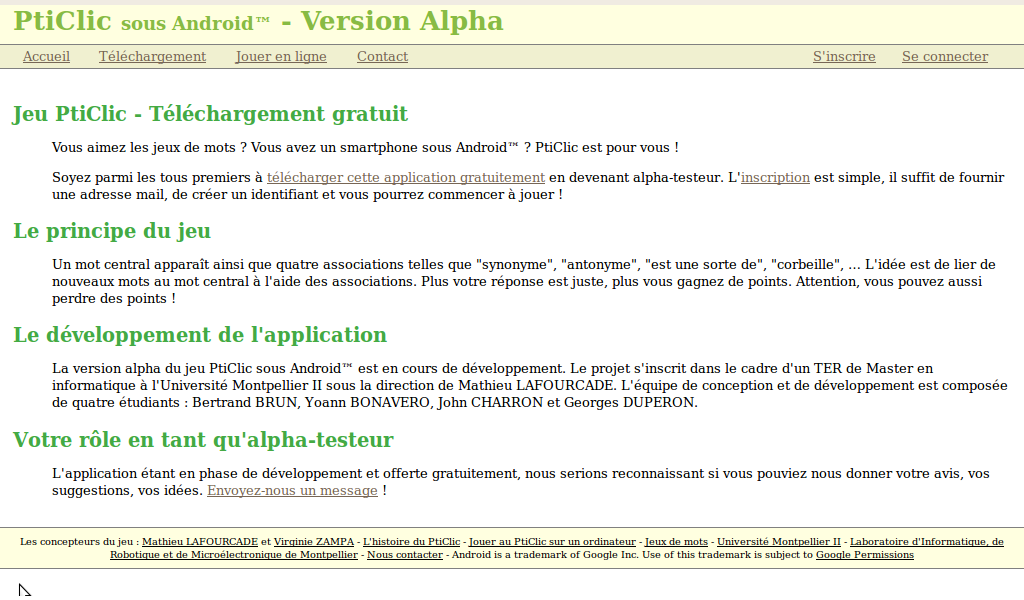
\includegraphics[width=14cm]{img/siteAccueil.png}
\end{center}

Dans les parties suivantes, les différentes pages de notre site seront décrites. 



\subsubsection{Téléchargement}

\begin{center}
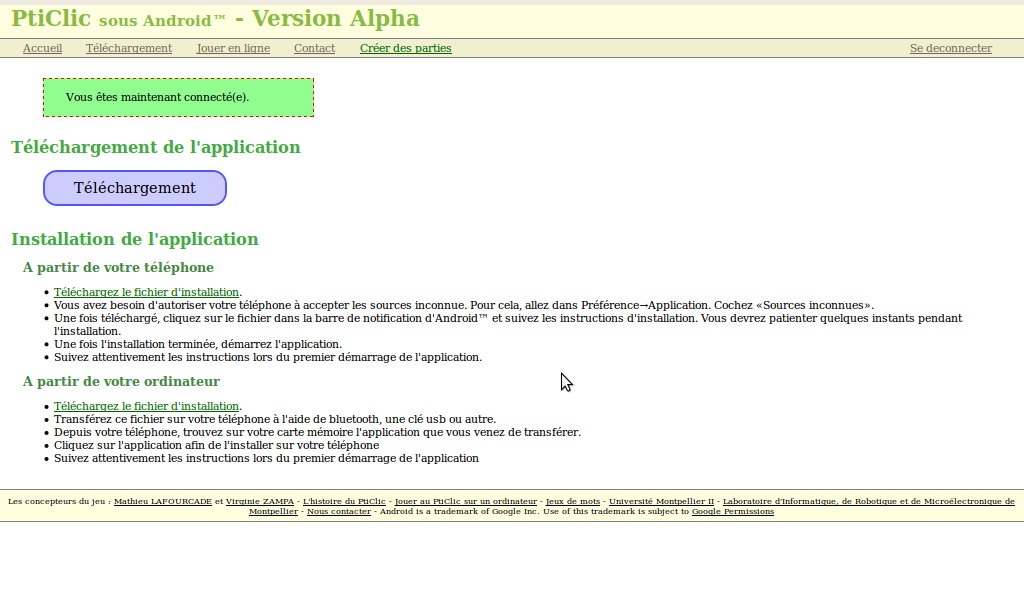
\includegraphics[width=14cm]{img/siteTelechargement.png}
\end{center}

La page 'Téléchargement' contient des instructions pour installer l'application Android de PtiClic. L'application peut être télécharger directement à partir d'un téléphone ou bien par le biais d'un ordinateur classique. 

Quant à la version HTML5, aucune installation est nécessaire, mais il est nécessaire de s'inscrire et s'authentifier afin d'y jouer. 

\subsubsection{L'inscription}
Si une personne est intéressée par notre jeu et qu'il souhaite y jouer, il devra tout d'abord s'inscrire afin qu'il
soit reconnu par le système. Cette opération est réalisée à partir du site à l'aide d'un formulaire comportant
trois informations obligatoires~: 'nom d'utilisateur', 'mot de passe' et 'mail'. Le formulaire se limite à champs (deux champs 'mot de passe') pour éviter de décourager les utilisateurs de s'inscrire.

\begin{center}
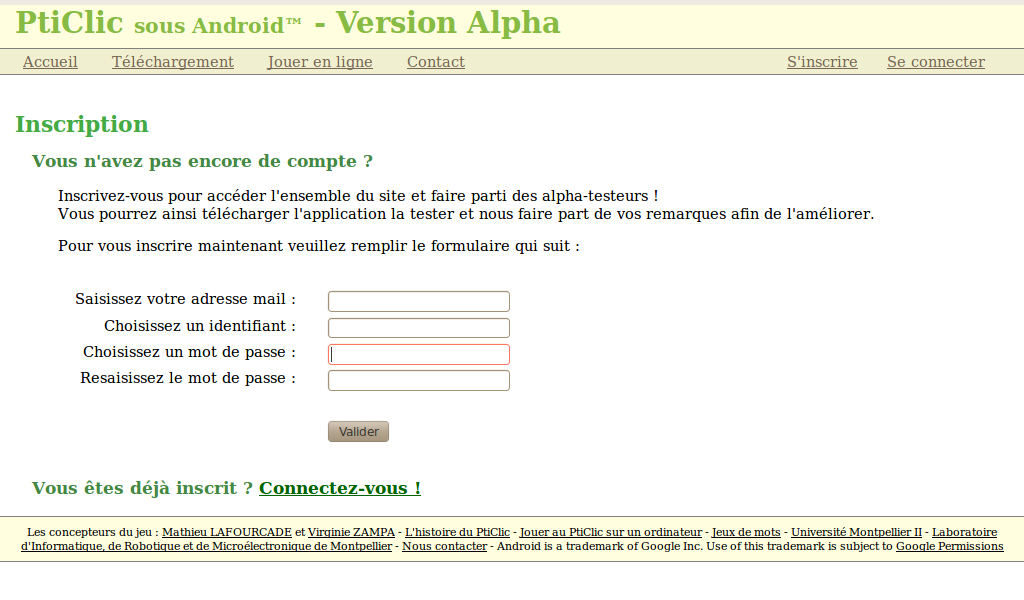
\includegraphics[width=14cm]{img/siteInscription.png}
\end{center}

L'inscription se réalise la première fois qu'un internaute souhaite jouer au jeu~; lorsque l'on essayé de jouer au jeu sans être authentifié, on est invité soit à s'identifier soit à s'inscrire et l'utilisateur choisit selon le cas qui lui convient. L'inscription, une fois faite, définitive, permet aux utilisateurs de jouer librement et peuvent comparer leur performances à d'autres joueurs.

\subsubsection{Contact}
Pour qu'une application soit en accord avec ses utilisateurs, il faut un certain temps et apporter un certain nombre
de modifications pour répondre à la demande et aux besoins de l'utilisateur final. Dans le but de récupérer les avis positifs et négatifs, les remarques et les critiques des utilisateurs, un formulaire de contact est disponible sur le site. 

\begin{center}
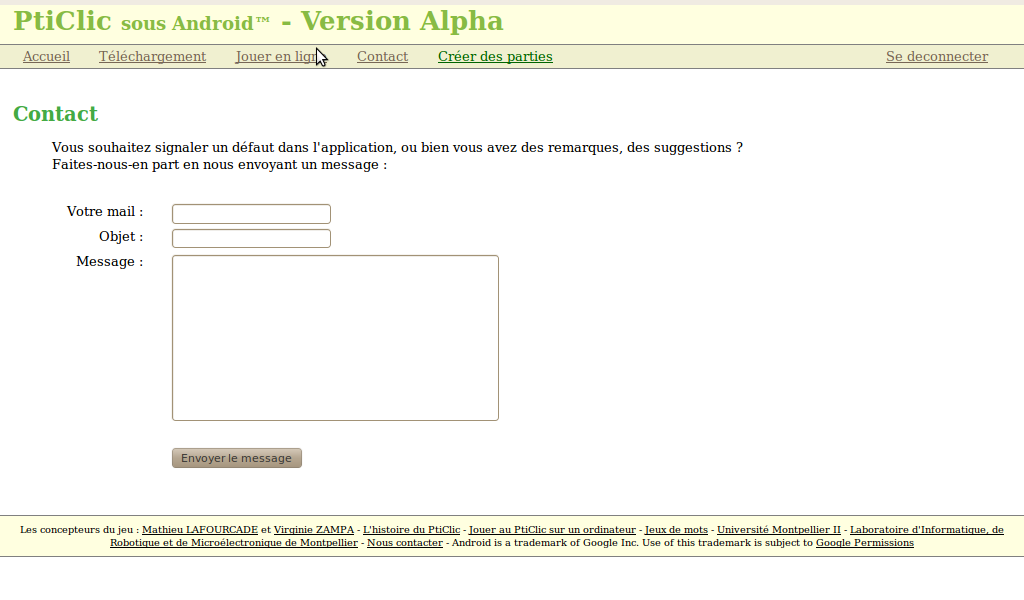
\includegraphics[width=14cm]{img/siteContact.png}
\end{center}

Ce formulaire est accessible sans inscription, ce qui permet d'envoyer un message s'il y a un problème lors de l'inscription au l'authentification, pour signaler un bogue concernant le site ou pour faire d'autres commentaires d'ordre général.

\subsubsection{La création de parties}
Un algorithme automatique de création de parties permet de créer un grand nombre de parties. Cependant, ce moyen
de génération de partie est assez limité et donne régulièrement des résultat trop peu satisfaisant voire même incohérents.

Pour palier à ce problème, une solution est de mettre en place un service permettant non pas à la machine, mais à des joueurs de créer eux-même des parties. Grâce à cette page, il est dorénavant possible d'obtenir des parties bien plus intéressantes, des parties qui contiennent un lexique spécifique à un domaine bien précis si le joueur est spécialiste d'un domaine précis ou bien des parties contenant de l'humour, par exemple. 


\begin{center}
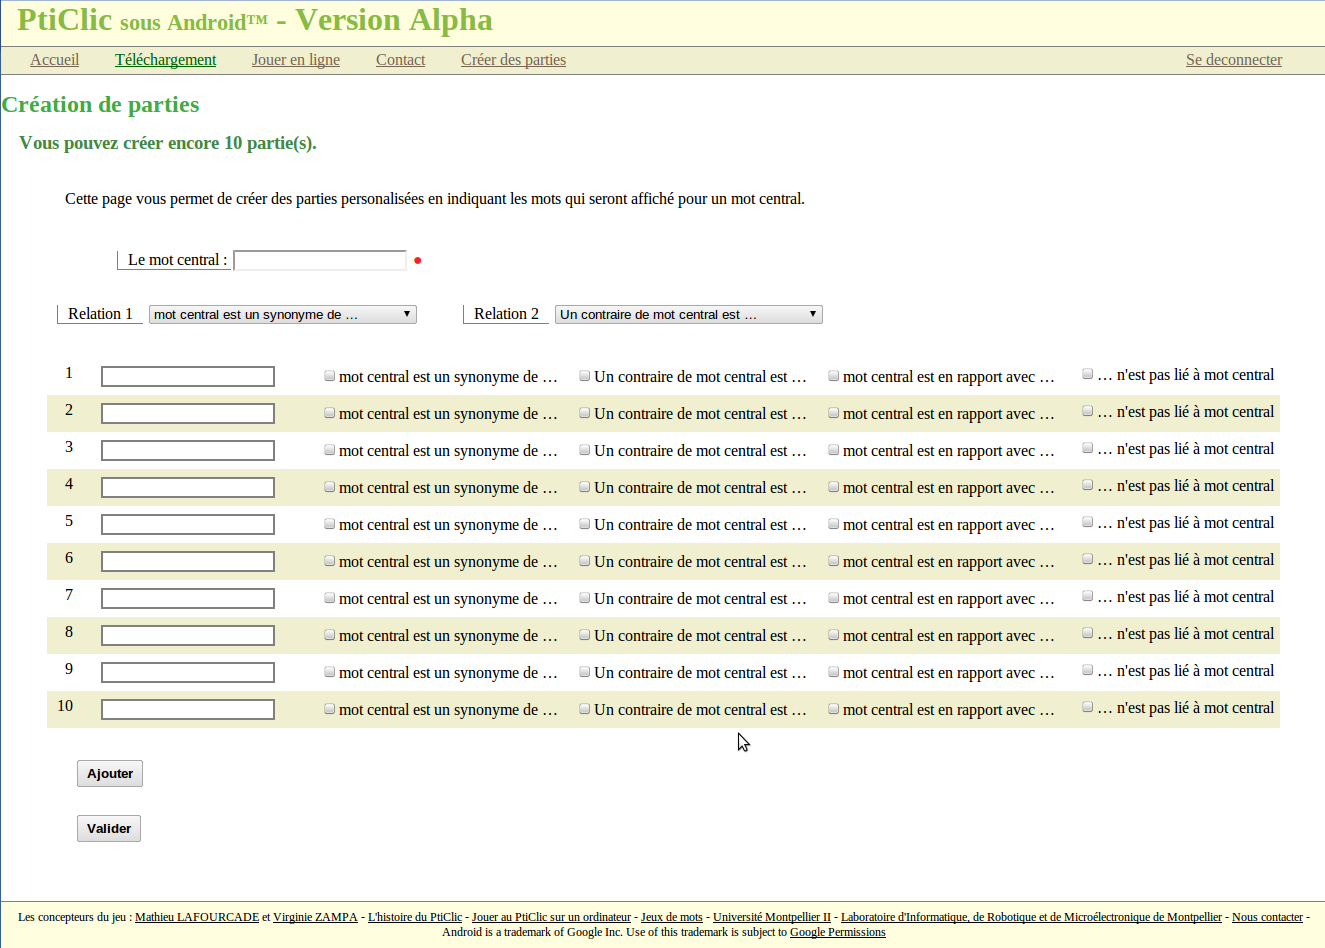
\includegraphics[width=14cm]{img/siteCreerParties.png}
\end{center}

Cette page permet de créer des parties de taille et de thèmes variés. Les joueurs peuvent choisir des mots ou des expressions qu'ils souhaitent voir dans une partie ainsi que deux relations principales.
Outre l'attractivité et l'intérêt de cette fonctionnalité, le joueur est mis en valeur du fait qu'il participe non seulement en tant que joueur, mais en tant que contributeur au projet. Les parties ainsi créées sont jouées par d'autres joueurs, améliorent la qualité des parties et le créateur et il serait même envisageable dans une future version de l'application de tenir le créateur de la partie au courant des joueurs qui ont joué sa partie et les scores obtenus.

La partie création de partie a été développé en JavaScript au lieu de PHP, ce qui a permis d'avoir une interaction en temps avec l'utilisateur. En effet, lorsqu'un utilisateur saisit un mot ou expression, il est important pour lui de savoir si ce mot existe ou non. De ce fait, une requête est émise en direction du serveur afin de vérifier la validité du mot ou expression saisi. Lorsqu'un utilisateur souhaite créer une nouvelle partie 
il ne sais pas forcément combien de mots va composer sa partie. Il devra par conséquent être en mesure d'augmenter au besoin le nombre de mots composants la partie.

\subsubsection{Jouez en ligne~!}
La seconde évolution majeure concernant le deuxième prototype du jeu est qu'il est possible de jouer directement depuis
le site Internet sans forcément disposer de téléphone sous \android{}. Cette option permet de toucher un public bien plus large sans pénaliser ceux qui disposent d'un smartphone \android{}

Une page du site Internet sera donc consacrée
à la création manuelle de partie. Elle permetra de créer des parties de taille variée et de thème différents. Le joueurs pourra
indiquer les mots qu'il souhaites voir dans la partie ainsi que les deux relations principales.
Les parties ainsi créées pourront être jouées par les autres joueurs et permettrons d'améliorer l'attractivité et l'intérêt du jeu.


\subsection{Version html5 du jeu}
\label{sec:html5}
\subsubsection{Architecture}

La version HTML5 du jeu  comporte 6 écrans~:
\begin{itemize}
\item Le «splash» au démarrage;
\item L'éran d'accueil, avec des liens vers les 4 autres (sauf score);
\item L'écran du jeu, avec le mot central, le mot du nuage et les quatre relations;
\item Le score, affiché à la fin de la partie;
\item Les préférences, qui permettent de choisir le thème de couleurs de l'application;
\item L'écran de connexion, sur lequel on peut se rendre depuis l'écran d'accueil, et qui s'affiche automatiquement lorsqu'on tente de faire
  une action (jouer ou modifier les préférences) sans être connecté;
\item L'écran «À propos», qui explique l'origine du jeu.
\end{itemize}



\begin{figure}[h!]
  \centering
      
\includegraphics[width=0.3\textwidth]{img/phone-splash.png}
  \caption{Le «splash» au démarrage}
\end{figure}

\begin{figure}[h!]
  \centering
      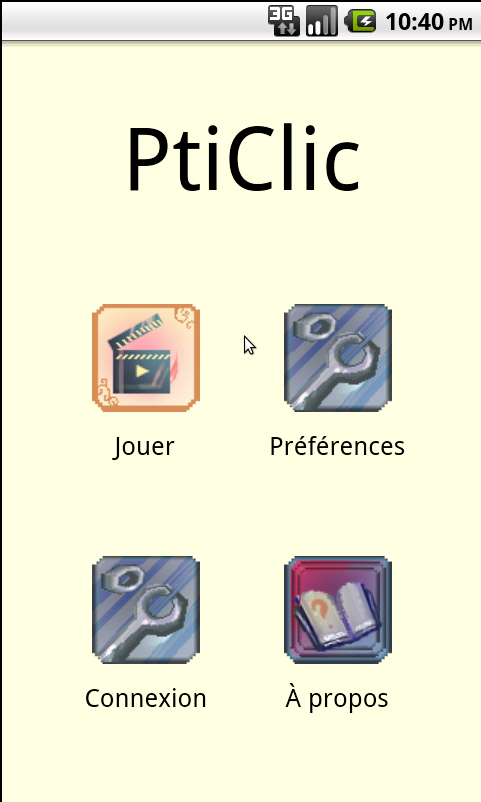
\includegraphics[width=0.3\textwidth]{img/phone-frontpage-deco.png}
  \caption{L'éran d'accueil, avec des liens vers les quatre autres (sauf score)}
\end{figure}

\begin{figure}[h!]
  \centering
      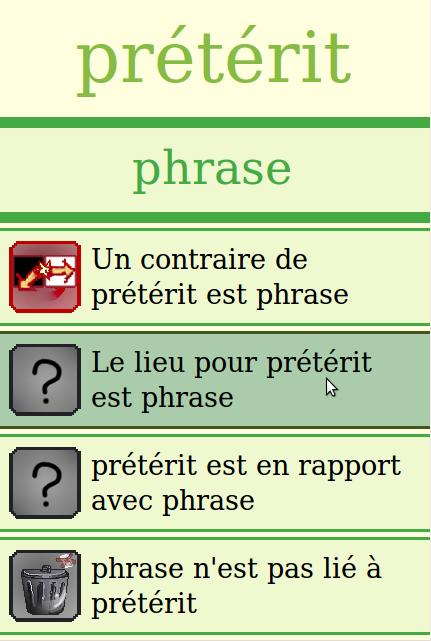
\includegraphics[width=0.3\textwidth]{img/preterit02.jpg}
  \caption{L'écran du jeu, avec le mot central, le mot du nuage et les quatre relations}
\end{figure}

\begin{figure}[h!]
  \centering
      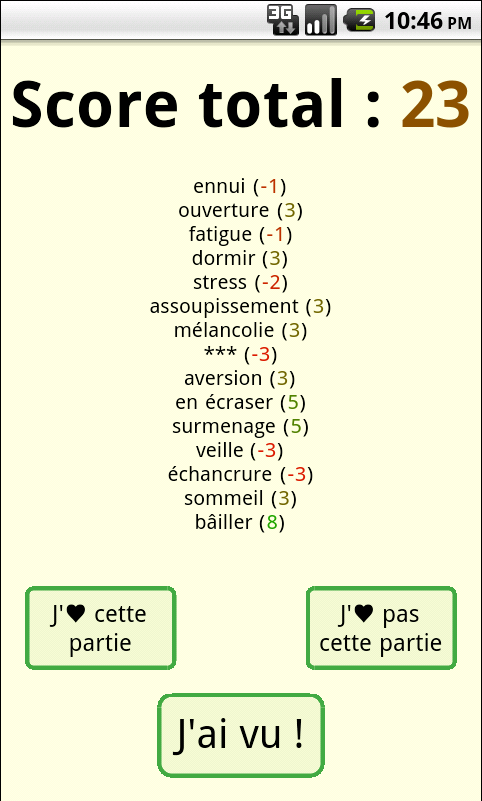
\includegraphics[width=0.3\textwidth]{img/phone-score.png}
  \caption{Le score, affiché à la fin de la partie}
\end{figure}

\begin{figure}[h!]
  \centering
      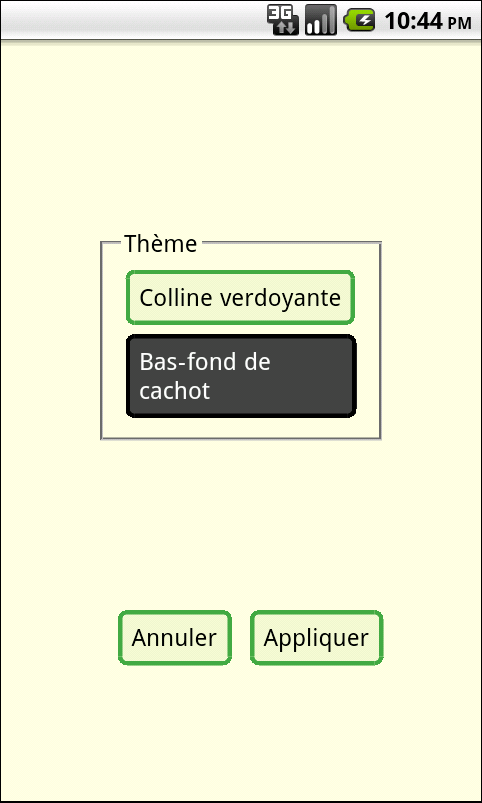
\includegraphics[width=0.3\textwidth]{img/phone-preferences.png}
  \caption{Les préférences, qui permettent de choisir le thème de couleurs de l'application}
\end{figure}

\begin{figure}[h!]
  \centering
      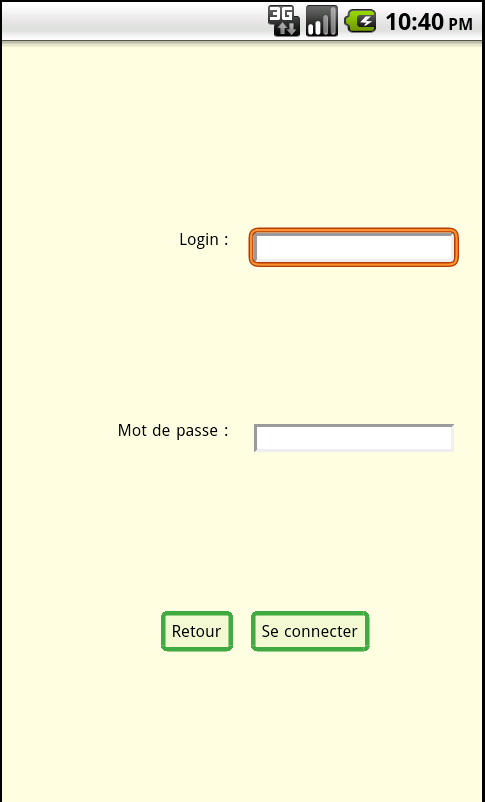
\includegraphics[width=0.3\textwidth]{img/phone-cnx.png}
  \caption{L'écran de connexion, sur lequel on peut se rendre depuis l'écran d'accueil, et qui s'affiche automatiquement lorsqu'on tente de faire}
\end{figure}


\begin{figure}[h!]
  \centering
      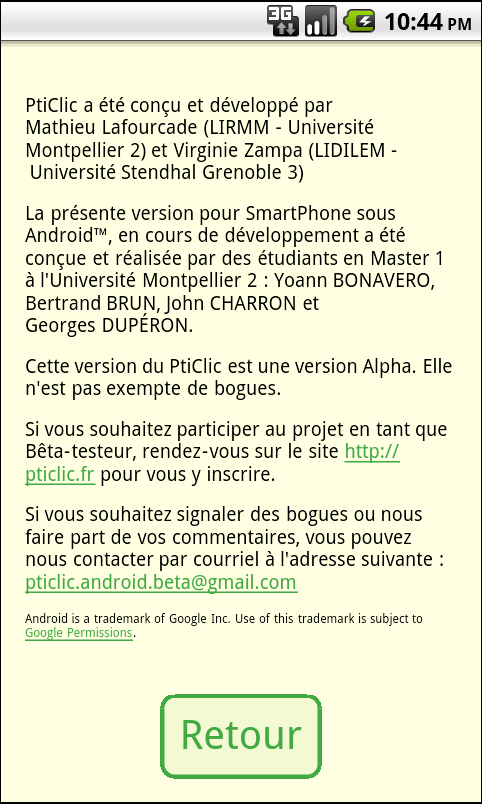
\includegraphics[width=0.3\textwidth]{img/phone-info.png}
  \caption{L'écran «À propos», qui explique l'origine du jeu}
\end{figure}


Chaque écran est contenu dans un élément HTML (\verb!<div/>!) qui est affiché uniquement lorsque l'utilisateur est sur cet écran.

La navigation entre les écrans et entre chaque mot du nuage lorsqu'on joue s'effectue en modifiant l'identifiant de fragment
de l'URL, c'est à dire la partie après le \verb!#!. De cette manière, chaque état est stocké dans l'historique du navigateur, et on peut revenir à
l'écran précédant à l'aide des boutons «Précédent» et «Suivant» classiques. De plus, cela permet d'annuler le choix d'une relation pour
un mot donné simplement en cliquant sur «Précédent».

L'état du programme -- écran en cours, thème de couleurs, structure de données représentant la partie en cours lorsqu'elle a été récupérée et de même pour les scores -- est stocké dans une variable nommée \verb!runstate!. Cependant, si l'on considère l'enchaînement d'actions
suivantes, on se rend compte qu'il doit y avoir une décorrelation entre l'état du programme tel que dictée par l'URL et l'état réel du
programme~:

\begin{itemize}
\item L'utilisateur clique sur «Jouer», ce qui l'amène à l'URL \verb!#game!;
\item L'écran de connexion est affiché pour que l'utilisateur s'identifie sans modifier l'URL (pour ne pas enregistrer cette étape
  transitoire dans l'historique).
\item Une fois l'utilisateur connecté, la partie commence.
\end{itemize}

Cette décorrelation apporte une certaine complexité au code de transition entre les états du programme, d'autant plus que l'application
effectue des requêtes réseau asynchrones, par exemple pour récupérer la partie durant lesquelles n'importe quelle séquence «Précédent» /
«Suivant» ou de modification arbitraire peut avoir lieu. Ainsi, entre le moment où l'on effectue une requête pour récupérer une nouvelle
partie et le moment où cette requête aboutit, l'utilisateur peut avoir cliqué sur «Précédent», ce qui le ramène à l'écran d'accueil (auquel
cas il ne faut pas afficher la partie lors de la réception), mais il peut aussi après ce «Précédent» faire «Suivant», auquel cas on se
retrouve de nouveau sur l'écran du jeu, et il faut donc afficher la partie lors de sa réception (et ne pas faire une deuxième requête
puisqu'il y en a déjà une en cours).

Pour gérer cela, nous avons implémenté une routine de transition entre les états qui envoie la séquence de messages suivante au nouvel
écran~:
\begin{itemize}
\item «goto», qui envoie le message «leave» à l'écran en cours, met à jour la variable runstate.screen, et communique quelques informations
  à l'application hôte en Java sous Android
\item «pre-enter», qui permet à l'écran d'effectuer des requêtes réseau avant son affichage;
\item «enter», qui affiche l'écran, et modifie dynamiquement son contenu si nécessaire (par exemple affichage du texte décrivant les
  relations dans l'écran du jeu)
\item «update» appellée une première fois juste après l'affichage de l'écran et à chaque changement d'URL qui ne modifie pas l'écran. Cela
  permet par exemple à l'écran du jeu de détecter qu'une réponse a été donnée pour un des mots du nuage et d'afficher le mot suivant.
\end{itemize}

Un changement d'URL déclenche donc soit un «goto», soit un «update», ce qui permet d'afficher l'écran voulu, tandis que les écrans peuvent
s'envoyer les uns les autres ces messages (principalement le message «goto») pour basculer de l'un à l'autre sans modifier l'URL.

\subsubsection{Concepts et techniques de programmation}

Les actions à déclencher lors de la réception du résultat d'une requête réseau ainsi que le cache partiel des parties et des scores (qui
permet de ne pas renvoyer une requête qui est déjà en cours ou a déjà abouti) sont implémentés en utilisant le paradigme de programmation
fonctionelle avec évaluation paresseuse, le côté «évaluation paresseuse» étant émulé en encapsulant le code dans des fonctions anonymes
(lambda fonctions).

Nous avons aussi employé une forme limitée de programmation réactive pour le cache, implémentée via l'objet \verb!Deferred! de JQuery.

Enfin, nous avons utilisé les capactités de JavaScript lui-même, qui est un langage objet basé sur les prototypes (et non les classes) pour
étendre le langage là où cela s'est avéré nécessaire.

\subsubsection{API Client-serveur}
Le client et le serveur utilisent tout deux une API qui permet de facilement remplacer un des deux composants. Tous les appels au serveur se font en HTTP GET et peuvent avoir les deux paramètres \verb!user! et \verb!password!. De plus, elles peuvent renvoyer une erreur au format suivant~:
\begin{alltt}
\{"error":\textit{Code d'erreur}, "msg":\textit{Message d'erreur}, "isError":true\}
\end{alltt}

Voici les principaux messages que supporte le serveur~:
\begin{itemize}
\item Récupérer une partie jouable~:

\verb!server.php?action=0!
{
\small
\begin{alltt}
\{
\quad"author":"\textit{Créateur de la partie}",
\quad"gid":\textit{Numéro de la partie},
\quad"pgid":\textit{Numéro de la partie jouable},
\quad"relations":[
\quad\quad\{"id":7,"name":"Un contraire de %mc est %mn"\},
\quad\quad…
\quad],
\quad"center":\{"id":\textit{eid mot central},"name":"\textit{Mot central}"\},
\quad"cloud":[
\quad\quad\{"id":\textit{eid mot nuage},"name":"\textit{Mot nuage}"\},
\quad\quad…
\quad]
\}
\end{alltt}
}
\item Répondre à une partie~:

\verb!server.php?action=1&gid=!\textit{\texttt{numéro de partie}}\verb!&pgid=!\textit{\texttt{numéro de partie}}

Cette requête doit aussi prendre un couple \textit{\texttt{numéro du mot du nuage}}\verb!=!\textit{\texttt{numéro de la relation}} pour
chaque réponse. Elle renvoie la structure suivante~:
{
\small
\begin{alltt}
\{
\quad"scoreTotal":\textit{Score pour la partie},
\quad"alreadyPlayed":\textit{true si la partie a déjà été jouée, false sinon},
\quad"author":\textit{Créateur de la partie}",
\quad"minScore":\textit{Plus petit score pour un mot},
\quad"maxScore":\textit{Plus grand score pour un mot},
\quad"newGame":\textit{Nouvelle partie, même format que action=0},
\quad"scores":[
\quad\quad\{"name":"\textit{Mot nuage}", "score":\textit{Score pour le mot}\}
\quad]
\}
\end{alltt}
}

\item D'autres actions de moindre intérêt sont disponibles, et permettent de~:
\begin{description}
\item[\verb!action=2!] Déclencher la création automatique de parties
\item[\verb!action=3!] Vérifier si un couple utilisateur/mot de passe est valide
\item[\verb!action=4!] Vérifier si un mot existe dans la base de données
% N°5 :
\item[\verb!action=5!] Récupérer la liste des relations disponibles («fait partie de», «synonyme»…)
\item[\verb!action=6!] Stocker une partie créée manuellement
\item[\verb!action=7!] Récupérer les préférences de l'utilisateur
\item[\verb!action=8!] Modifier les préférences de l'utilisateur
\item[\verb!action=9!] Terminer la session et déconnecter l'utilisateur
% n°10 :
\item[\verb!action=10!] Indiquer si l'utilisateur aime ou non la partie à laquelle il a joué.
\end{description}

\end{itemize}


\subsection{Algorithmes de création du nuage}

(voir aussi la partie 4)

Pour construire le nuage de mots à partir d'un mot central et de deux relations, nous avons étudié les algorithmes suivants.

\subsubsection{Mots à proximité}
\begin{figure}[ht]
  \begin{center}
    \begin{tikzpicture}[
      mynode/.style = {circle, minimum size=1.5cm},
      mc/.style = {mynode,draw=red,text=red},
      mn/.style = {mynode,draw},
      mi/.style = {mynode,draw=gray,text=gray},
      rel/.style = {font=\footnotesize},
      guess/.style = {->,dashed},
      exist/.style = {->},
      auto,swap
      ]
      \node[mc] (mc) {Chat};
      \node[mn] (mn0) at (0,3) {Souris};
      \node[mi] (mi1) at (3,-2) {matou};
      \node[mn] (mn2) at (6,0) {animal};
      \node[mn] (mn3) at (-3,-2) {félin};
      \path[exist] (mc) edge[bend right] node[rel]{idée associée} (mn0);
      \path[exist] (mc) edge node[rel]{synonyme} (mi1);
      \path[exist] (mi1) edge node[rel]{sorte de} (mn2);
      \path[guess,swap] (mc) edge node[rel]{sorte de ?} (mn2);
      \path[guess,swap] (mc) edge[bend left] node[rel]{\shortstack{sorte de ?\\synonyme ?\\\dots}} (mn0);
      \path[exist] (mn3) edge[bend right] node[rel]{spécifique} (mc);
      \path[guess] (mc) edge[bend right] node[rel]{sorte de ?} (mn3);
    \end{tikzpicture}
    \caption{Algorithme de création d'un nuage de mot par sélection des mots proches du mot central.}
    \label{fig:algo-proximite}
  \end{center}
\end{figure}

Cet algorithme (Fig. \ref{fig:algo-proximite}) sélectionne des mots proches du mot central en empruntant~:
\begin{itemize}
\item La relation «Idée Associée», pour la spécialiser;
\item Des relations qui «entrent» dans le mot central;
\item Un enchaînement de deux relations. Dans ce dernier cas, le fait qu'une des deux relations soit «Sysnonyme» est privilégié.
\end{itemize}

Cet algorithme a donné de bons résultats après que nous ayons filtré les mots centraux pour ne prendre en compte que ceux dont le nombre de
relations sortantes dépassaient un certain seuil, de manière à s'assurer qu'ils auraient suffisemment de liens pour pouvoir construire un
nuage intéressant. De plus, nous avons pondéré la fréquence à laquelle les différentes méthodes (arc avant, arc arrière, enchaînement de
deux arcs) étaient utilisées, de manière à avoir plus de mots du nuage pertinants.

L'avantage de cet algorithme est d'avoir une assez grande couverture du voisinage du mot central et la possibilité de raffiner les
relations («Idée Associée» vers une autre relation par exemple). Un inconvénient est que les relations proposées ne sont pas toujours
pertinantes (relation «sorte de» pour des verbes par exemple). De plus, l'algorithme pourra proposer en déduction de l'enchaînement de deux
relation une relation quelconque, qui ne sera pas forcément logique par rapport aux deux autres.

Pour résoudre ce dernier défaut, nous avons élaboré un autre algorithme.

\subsubsection{Algorithme des «triangles»}
\begin{figure}[ht]
  \centering
  \begin{center}
    \begin{tikzpicture}[
      mynode/.style = {circle, minimum size=1.5cm},
      mc/.style = {mynode,draw=red,text=red},
      mn/.style = {mynode,draw},
      mi/.style = {mynode,draw=gray,text=gray},
      rel/.style = {font=\footnotesize},
      guess/.style = {->,dashed},
      exist/.style = {->},
      auto
      ]
      \node[mc] (mc) {Mot central};
      \node[mi, above right=of mc] (mi) {Intermédiaire};
      \node[mn, below right=of mi] (mn) {Mot nuage};
      
      \path[draw,->] (mc) edge node {Relation 1} (mi);
      \path[draw,->] (mi) edge node {Relation 2} (mn);
      \path[draw,->] (mc) edge node[swap] {Relation déduite} (mn);
    \end{tikzpicture}
  \end{center}
  \caption{Une relation déductible grâce aux deux autres}
  \label{fig:algo-triangles}
\end{figure}

Cet algorithme (Fig. \ref{fig:algo-triangles}) compte le nombre de «triangles» (cliques composées de trois noeuds) que l'on peut trouver
dans les relations existantes, pour un triplet de relations donné, et le divise par le nombre d'occurences des deux côtés du triangle (du
mot central au mot intermédiaire, et du mot intermédiaire au mot nuage), sans prendre en compte le troisième côté. Cela permet d'associer à
chaque triplet de relations la probabilité qu'on puisse déduire la troisième à partir des deux autres.

La génération du nuage se déroule alors de la manière suivante~: On sélectionne tous les mots que l'on peut atteindre par l'enchaînement de
deux relations, et on les inclue dans le nuage en fonction de la probabilité qu'on puisse déduire une des deux relations de la partie en
utilisant les deux relations empruntées.

Cette technique est équivalente à l'utilisation d'un réseau de neurones (Fig. \ref{fig:reseau-neurones}) pour classifier les mots du nuage
parmi les différentes relations disponibles.

\begin{figure}[ht]
  \begin{center}
    \begin{tikzpicture}[
      node/.style={draw,ellipse,font=\footnotesize, minimum width=3cm, minimum height=0.7cm},
      hidden/.style={minimum width=4cm}
      ]
      \node[node,anchor=east] (R1) at (-3.5,1.2) {Type relation 1};
      \node[node,anchor=east] (R2) at (-3.5,-1.2) {Type relation 2};
      \node[node, hidden] (H1) at (0,2.4) {$R1 = 5 \wedge R2 = 5$};
      \node[node, hidden] (H2) at (0,1.2) {$R1 = 5 \wedge R2 = 7$};
      \node[node, hidden] (H3) at (0,0) {…};
      \node[node, hidden] (H4) at (0,-1.2) {$R1 = 22 \wedge R2 = 13$};
      \node[node, hidden] (H5) at (0,-2.4) {$R1 = 22 \wedge R2 = 22$};
      \node[node,anchor=west] (R31) at (3.5,1.2) {Synonyme};
      \node[node,anchor=west] (R32) at (3.5,0) {Contraire};
      \node[node,anchor=west] (R33) at (3.5,-1.2) {…};
      
      \foreach \hidden in {H1,H2,H3,H4,H5}{
        \draw (R1.east) -- (\hidden.west);
        \draw (R2.east) -- (\hidden.west);
      }
      \foreach \hidden in {H3,H4,H5}{
        \draw (\hidden.east) -- (R31.west);
        \draw (\hidden.east) -- (R32.west);
        \draw (\hidden.east) -- (R33.west);
      }
      \draw[draw=green!50!black] (H1.east) edge node[near start,text=green!50!black] {1} (R31.west);
      \draw[draw=red] (H2.east) edge node[near start,text=red] {0} (R31.west);
      \draw[draw=red] (H1.east) edge node[near start,text=red] {0} (R32.west);
      \draw[draw=green!50!black] (H2.east) edge node[near start,text=green!50!black] {1} (R32.west);
      \draw (H1.east) -- (R33.west);
      \draw (H2.east) -- (R33.west);
    \end{tikzpicture}
    \caption{Réseau de neurones pour la classification des mots du nuage parmi les relations disponibles, en fonction des arcs qui les
      ratachent au mot central.}
    \label{fig:reseau-neurones}
  \end{center}
\end{figure}

Les probabilités recueillies par l'algorithme décrit ci-dessus correspondent à la valeur de sortie des neurones de la couche interne, et les
types des relations sur les deux premiers arcs correspondent à la fonction d'activation de ces mêmes neurones. Pour chaque type du troisième
arc, on a une catégorie en sortie du réseau de neurones.

Par exemple, sur la figure \ref{fig:reseau-neurones}, sachant que la relation 5 est «Synonyme» et la relation 7 «Contraire», le premier
neurone de la couche interne s'active si les deux relations qui relient le mot central au mot du nuage sont toutes deux «Synonyme». Sa
valeur de sortie pour la catégorie «Synonyme» est alors proche de 1 (le synonyme d'un synonyme est souvent un synonyme), tandis que sa
valeur pour la catégorie «Contraire» est proche de 0 (le contraire d'un synonyme est un contraire, pas un synonyme).

Cet algorithme a donné d'excellents résultats pour les relations qui pouvaient se déduire avec de fortes probabilités, cependant bon nombre
de relations ne s'appliquent à des mots n'appartenant qu'à une partie du discours donnée (nom, adjectif, verbe…), et la probabilité de les
voir apparaître en déduction de deux autres était très faible.

\subsubsection{Algorithme des «triangles» avec les parties du discours}

Nous avons donc élaboré une variante (Fig. \ref{fig:algo-triangles-pos}) de cet algorithme qui prenait en compte les parties du discours
(Part Of Speach) auxquelles appartenaient les noeuds.

\begin{figure}[ht]
  \centering
  \begin{center}
    \begin{tikzpicture}[
      mynode/.style = {circle, minimum size=1.5cm},
      mc/.style = {mynode,draw=red,text=red},
      mn/.style = {mynode,draw},
      mi/.style = {mynode,draw=gray,text=gray},
      rel/.style = {font=\footnotesize},
      guess/.style = {->,dashed},
      exist/.style = {->},
      auto
      ]
      \node[mc] (mc) {\shortstack{Mot central\\POS 1}};
      \node[mi, above right=of mc] (mi) {\shortstack{Intermédiaire\\POS 2}};
      \node[mn, below right=of mi] (mn) {\shortstack{Mot nuage\\POS 3}};
      
      \path[draw,->] (mc) edge node {Relation 1} (mi);
      \path[draw,->] (mi) edge node {Relation 2} (mn);
      \path[draw,->] (mc) edge node[swap] {Relation déduite} (mn);
    \end{tikzpicture}
  \end{center}
  \caption{Une relation déductible grâce aux deux autres}
  \label{fig:algo-triangles-pos}
\end{figure}

Le probleme qui s'est alors posé, est que'avec environ 12 parties du discours différentes, et 16 relations différentes, le nombre de
6-uplets distincts dans l'ensemble $POS^3\times Rel^3$ s'élevait à plus de 7 millions. Cela signifie que nous avions plus de 7 millions de
«types» de triangles à considérer, alors que seulement peu d'entre eux montraient une réelle possibilité de déduction. De plus, il n'y a
dans la base de données qu'environ un million de relations existantes, nous nous trouverions donc dans une situation de surapprentissage.

Ce problème montre la nécessité d'étudier manuellement quelles parties du discours ont un intérêt pour quelles relations, afin de réduire
l'espace des 6-uplets constitués des parties du discours des noeuds et des types de relations formant les arcs qui permettent la déduction
du dernier arc.


\subsection{Protection contre les attaques des joueurs}

Le serveur prévient quelques types d'attaques que des joueurs pourraient effectuer pour améliorer leur score. Entre autres, lorsqu'un joueur
a envoyé ses réponses à une partie et que ses scores lui ont été envoyés, la modification des réponses est refusée s'il tente de renvoyer
d'autres réponses. Cela permet d'éviter qu'un joueur améliore son score en donnant les réponses attendues une fois qu'il les connaît.

Nous n'avons cependant pas de protection contre un utilisateur qui donnerait exprès les mauvaises réponses (une forme de SPAM qui influerait
la base de données). La détection de ce comportement est difficile car il est tout à fait possible que les réponses que notre algorithme
estime être les bonnes soient justes et il est tout à fait légitime qu'un utilisateur soit en désacord avec les uns avec les autres.

Dans le cas de l'utilisation d'un robot pour donner en masse de mauvaises réponses, il serait possible de détecter la fréquence élevée des
parties jouées, ce qui n'empêcherait cependant pas un robot de se créer plusieurs comptes pour éviter cette détection. De même que la
détection de courriers indésirables est difficile dans le cadre de la messagerie électronique, la détection de la transmission massive de
mauvaises réponses à notre serveur est compliquée, d'autant plus que peu de données sont transmises pour chaque partie.

\section{Discussion et conclusion}

Dès le début du projet, nous avons été confrontés à des difficultés techniques. L'émulateur \android{} qui devait nous permettre de tester
l'application lors du développement s'est révélé être extrêmement lent au point d'être inutilisable sur les ordinateurs de plusieurs des membres
du groupe. Pour contourner ce problème, nous avons installé l'émulateur sur les machines du RezUFR (bâtiments 5, 6 et 16), mais sa
configuration s'est avérée problématique, ce qui nous a fait perdre beaucoup de temps, pour finalement nous rendre compte que l'installation était plutôt instable.

En ce qui concerne le travail sur le serveur, la tâche a été compliquée par des erreurs de syntaxe (guillemets non échappés, etc.) dans
l'archive de la base de données qui nous a été fournie, ce qui nous a obligés à passer du temps à contourner ces erreurs avant de pouvoir
analyser la base de données. Pour cette analyse, le volume de données à traiter (base de données de plus de 100Mo) nous a ralentis lors de
l'élaboration de l'algorithme de création de parties.

Lors de la construction des requêtes utilisées dans le serveur, nous nous sommes confrontés à d'autres problèmes~:

SQLite3 n'est pas capable d'utiliser un index pour la requête extérieure sur une requête du type
\begin{verbatim}
select * from (select * from table where condition) where condition
\end{verbatim}
Il y a eu par conséquent nécessité de réécrire certaines requêtes avec des jointures a priori beaucoup moins efficaces, mais sont tout de même efficace grâce aux index.

SQLite3 tranforme les requêtes de la forme \verb!select * from table limit 100 order by random();! en une requête qui récupère tout le set
de résultats, ajoute une colonne random(), prend les 100 premiers résultats et les trie. Mais cela l'oblige à récupérer tout le set de
résultats et de calculer le random() pour chaque ligne, pour ensuite jeter tout ce qui dépasse la ligne 100. Cela est évidemment très coûteux
dans le cadre de requêtes avec beaucoup de résultats. Nous avons donc dû isoler la requête avec \verb!limit! de son \verb!order by! avec
des «hacks» assez tordus pour tromper l'optimiseur.

Lors du développement de l'application Java, le langage de description des interfaces utilisateur d'\android{}, qui est une application XML,
s'est montré peu pratique pour la construction de l'interface d'un jeu, et difficile à modifier pour de petits ajustements (ajout d'un
bouton, d'une icône…). C'est une des raisons pour l'abandon de la plateforme \android{} + Java, en faveur de HTML5 + CSS + JavaScript.

Dans l'application HTML5, l'omniprésence d'évènements asynchrones a été la source de nombreux bugs. De plus, des légères différences de
comportement entre le navigateur Web d'\android{} et les navigateurs sur les PC ont fait que certains problèmes ne se posaient que
sur le téléphonne physique, ce qui a rendu leur résolution difficile.

L'application pourrait bénéficier d'une restructuration du code. Nous avons effectué cette restructuration et un gros
nettoyage du code du client, mais le serveur n'est pas aussi propre et extensible que souhaitable.

Bien que fonctionnelle, notre application peut encore être améliorée. L'implémentation d'un des modes de jeu prévus au départ, par exemple
le mode «thématique», pourrait être couplé avec un mode «l'image cachée»~: on choisit un thème et au bout de plusieurs parties on découvre une
image associée à ce thème, ce qui contribuerait à l'addictivité du jeu.

Un autre aspect qui pourrait être amélioré est la qualité des nuages des mots générés. Actuellement, l'algorithme de génération des nuages ne tient pas
compte de la partie du discours à laquelle le mot central et les mots du nuage appartiennent. Par exemple, la relation «fait partie de» n'a
de sens que pour des noms, alors que notre algorithme peut aussi bien la choisir avec un adjectif comme mot central.

Nous avons pensé à utiliser une forme de réseau de neurones pour déterminer si un mot central et des mots du nuage sont pertinants pour une
relation donnée. Nous avons commencé à implémenter un tel algorithme, mais n'avons pas eu le temps terminer cette amélioration.

Un paquetage TALN séparé a été en cours de développement et les résultats sont prometteux, mais ce paquetage est toujours au stade expérimental et les classes qui étaient prévues d'être intégrées au projet n'ont pas vu le jour.


Le client et le serveur constituent tous les deux des briques logicielles réutilisables. Le serveur peut être réutilisé assez facilement
pour d'autres applications qui souhaiteraient afficher par exemple le nuage pour un mot donné. Le client communique avec le serveur en
utilisant seulement quelques types de requêtes différents et pourrait donc être couplés avec un autre serveur avec peu de modifications\footnote{nous pensons ici au serveur existant de la version de PtiClic réalisée par le LIRMM}.

Le client est aussi extensible~: son architecture permet l'ajout de nouveaux écrans, de nouveaux thèmes, voire de nouveaux modes de jeu. Le
fait qu'il soit écrit principalement en HTML5 et JavaScript permet de l'adapter à la plupart des téléphonnes intelligents et aux tablettes à
moindre coût.

Nous espérons que notre travail pourra être réutilisé par l'équipe du LIRMM pour offir une interface au jeu PtiClic qui soit compatible avec
les platesformes mobiles.

\newpage

\section{Bibliographie}
\subsection{PtiClic et TALN}

Lafourcade, Mathieu, Making people play for Lexical Acquisition. In Proc. SNLP 2007, 7th Symposium on Natural Language Processing. Pattaya, Thailande, 13-15 December 2007.

Lafourcade, Mathieu and Alain Joubert, Computing trees of named word usages from a crowdsourced lexical network. In proc Computational Linguistics Applications - International Multi-Conference on Computer Science and Information Technology, Wisla, Pologne, 18-20 October 2010.

Lafourcade, Mathieu and Alain Joubert, Détermination et pondération des raffinements d'un terme à partir de son arbre des usages nommés. In proc of TALN'10, Montreal, Canada, 19-23 Juillet 2010.

Lafourcade, Mathieu and Alain Joubert, JeuxDeMots : un prototype ludique pour l’émergence de relations entre termes. In proc of JADT'2008, Ecole normale supérieure Lettres et sciences humaines , Lyon, France, 12-14 mars 2008.

Lafourcade, Mathieu and Virginie Zampa, PtiClic~: a game for vocabulary assessment combining JeuxDeMots and LSA. In proc of CICLing (Conference on Intelligent text processing and Comptational Linguistics). Mexico : 1-7 mars 2009.

Lafourcade, Mathieu and Virginie Zampa, PtiClic et PtiClic-kids~: Jeux avec les mots permettant une double acquisition. In proc TICE 2010, 7e coloque TICE, Nancy~: 6-8 décembre 2010 et PtiClic: a game for vocabulary assessment combining JeuxDeMots and LSA. In proc of CICLing (Conference on Intelligent text processing and Comptational Linguistics). Mexico : 1-7 mars, 2010.

Schwab, Didier and Mathieu Lafourcade, Modelling, Detection and Exploitation of Lexical Functions for Analysis, ECTI Journal, 2007, Vol.2, No2, ISSN 1905-050X, pp 97-108.

Wikipedia, Latent Semantic Analysis http:\/\/en.wikipedia.org\/wiki\/Latent\_semantic\_analysis.

Wikipedia, Analyse sémantique latante, http:\/\/fr.wikipedia.org\/wiki\/Analyse\_s\%C3\%A9mantique\_latente.


\subsection{Linguistique}

Saussure, Ferdinand de, Cours de linguistique générale, édition originale~: 1916, édition 1979~: Payot, Paris. 


\subsection{Java}

Code Conventions for the Java Programming Language, Oracle, 1999. (\url{http://www.oracle.com/technetwork/java/codeconvtoc-136057.html, www.oracle.com/technetwork/java/codeconventions-150003.pdf})

\subsection{\android{}}

Android Developer, 2011. (\url{http://developer.android.com/})





% \section{Notes Georges}
% Les relations suivantes seront peut-être utilisées (* = oui, c'est sûr, on a/doit faire les icônes et des requêtes sql)~:

% \begin{tabular}{|c|l|l|l|}
% \hline
% icône~? & nom & num & signification \\
% \hline
% $*$ & r\_syn       & 5  & synonyme (chat -> matou) \\
% $*$ & r\_anto      & 7  & antonyme (bon -> mauvais) \\
% $*$ & r\_has\_part & 9  & A comme partie (chat -> patte) \\
% $*$ & r\_holo      & 10 & Fait partie de (patte -> chat) \\
%     & r\_agent     & 13 & Peut exécuter comme action (chat -> manger) \\
%     & r\_patient   & 14 & Peut subir comme action (chat -> laver) \\
%     & r\_carac     & 17 & Caractéristique (chat -> affectueux (ou pas…)) \\
% \hline
% \end{tabular}

\newpage

\appendix

\section{Diagramme de Gantt prévisionnel}
\label{sec:gantt-original}
\noindent
\hskip -2.6cm%
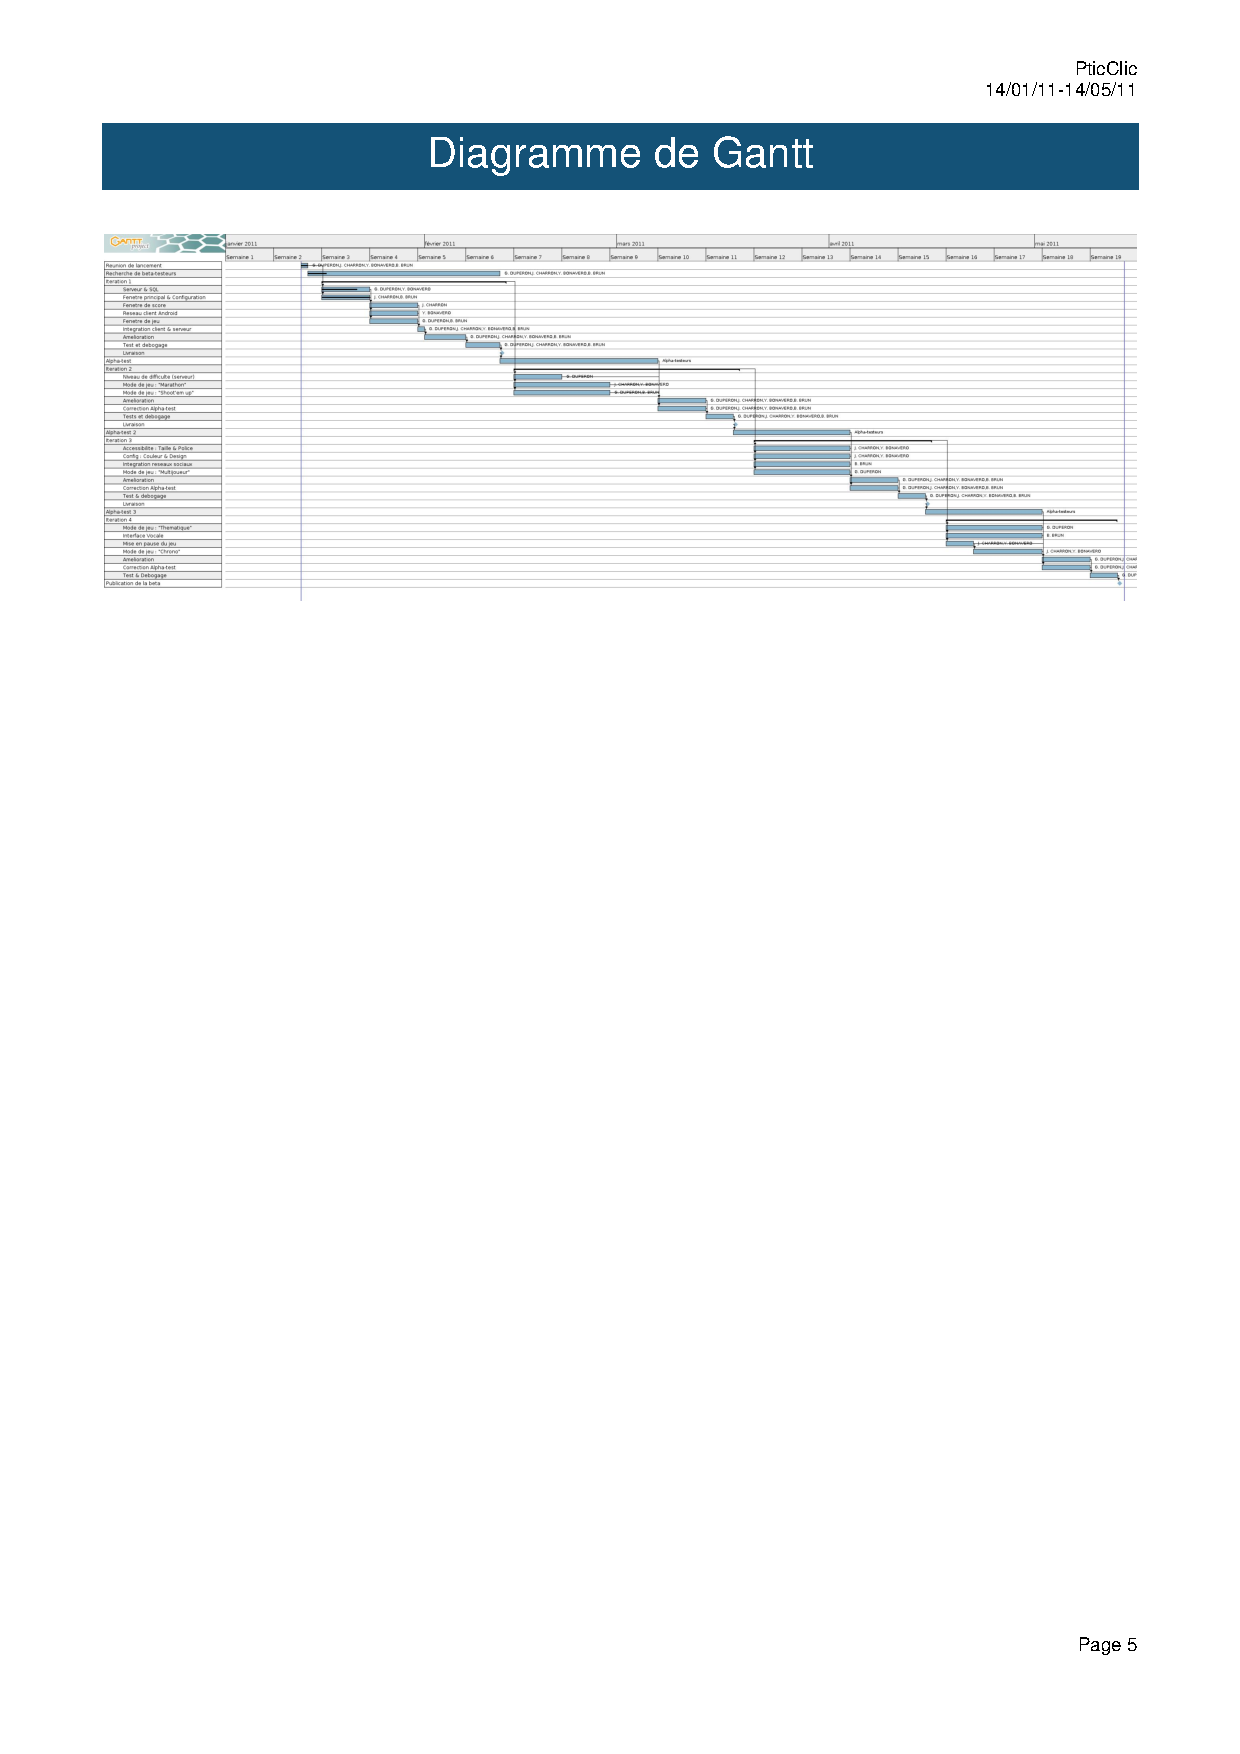
\includegraphics[trim=1.7cm 19cm 1.7cm 4cm,clip,width=20cm]{../feuille-route/gp-pticlic.pdf}
\newpage

% \section{Annexe A}

% \subsection{14 janvier 2010}

% Durée du projet 4 mois (4 itérations de 4 semaines)

% Conventions de code : \url{http://java.sun.com/docs/codeconv/html/CodeConventions.doc6.html}

% Code (noms de variables, etc.) en anglais, commentaires en français, javadoc en français.

% \subsection{26 janvier 2011}
% Mettre le serveur (PHP) sur free.fr, pour pouvoir tester facilement

% Utilisation d'une classe \verb!Constant!

% Écran d'accueil du jeu : Image (splash), puis directement les icônes des modes de jeu + configuration, au lieu d'avoir un écran avec le logo et jouer/config, suivi du choix du mode de jeu.

\section{Annexe A}

%\subsection{Serveur}

****SQL****
2011-m1s2-ter\/code\/serveur\$ ls
02122011-LEXICALNET-JEUXDEMOTS-FR-NOHTML.txt  -- dump de Lafourcade
dump.url -- contient l'URL du dump le plus récent
dump2mysql.sh -- Script pour convertir dump de Lafourcade en sql (pas terminé~? On utilise sqlite, donc on a laissé tombé~?)
dump2sqlite.sh  -- Script pour convertir dump de Lafourcade en sql
README.sh -- Ce n'est pas un README, c'est un script pour faire l'ensemble de la création de la BD, du téléchargement à la création d'indexes en passant par la création des tables et les insertions.
sql -- Le script sql à proprement parler
php\/db -- fichier binaire sqlite pour le chargement de la bd
php\/db.old -- fichier binaire sqlite pour le chargement de la bd, version précédente (backup)
dossier: select

****SERVEUR****
php\/db.php -- fichier pour ouvrir et fermer ou récupérer l'instance de l'ouverture de la base de données à l'aide d'un singleton. 
		Fichier très court, deux fonctions seulement.
php\/pticlic.php -- contient un grand nombre de fonctions pour le jeu
php\/relations.php -- contient un tableau et les phrases 'relation'
php\/server.php --



****SITE****
php\/contact.php
php\/createGame.php
php\/download.php
php\/index.php
php\/login.php
php\/showGame.php -- ??
php\/signup.php
php\/ressources/backend.css  -- CSS pour showGame.php
php\/ressources/footer.inc  -- pied de pages du site
php\/ressources/locations.inc  -- petit fichier facilitant la navigation de page en page
php\/ressources/menu.inc  -- menu du site
php\/ressources/pticlic-alpha-v0.1.apk  -- exécutable PtiClic (fichier d'installation de l'application)
php\/ressources/showmsg.inc  -- ?? (pour l'affichage des messages... mais dans quel contexte~? Pourquoi~?)
php\/ressources/simple.css  -- CSS de base du site
php\/ressources/strings.inc -- fichier de configuration des strings (phrases utilisés de manière répétitive dans le site, par exemple, les messages d'erreurs)

\section{Mentions légales}
Android is a trademark of Google Inc. Use of this subject to Google Permissions.


\end{document}
